\documentclass[letterpaper,twocolumn,10pt]{article}
\usepackage{usenix}

\usepackage{tikz}
\usepackage{amsmath}
\usepackage{amssymb}
\usepackage{xcolor}
\usepackage{booktabs}
\usepackage{url}
\usepackage[normalem]{ulem}
\usepackage{tikz}
\usetikzlibrary{positioning,arrows.meta,calc,fit}
\usetikzlibrary{positioning, decorations.pathreplacing}
\usepackage{booktabs,pifont,makecell}
\newcommand{\cmark}{\ding{51}}
\newcommand{\xmark}{\ding{55}}
\usepackage{amsthm}                 % Theorem 1 / Lemma 1 / Prop 1 + proof env
  \newtheorem{theorem}{Theorem}
  \newtheorem{lemma}{Lemma}
  \newtheorem{proposition}{Proposition}
  \theoremstyle{definition}
  \newtheorem{definition}{Definition}
  \newtheorem{assumption}{Assumption}
\usepackage{algorithm}              % Algorithm 1 (linear scan)
\usepackage{float}                  % [H] placement for the appendix component map
\usepackage{algpseudocode}          % Algorithm 2 (binary search)
\usepackage{booktabs}
\usepackage{colortbl}
% Self-wrapping (\ensuremath): each macro works in BOTH text and math mode, so
% e.g. \spl{t} in running text no longer needs enclosing $...$.
\providecommand{\run}{\ensuremath{\mathit{run}}}
\providecommand{\IS}{\ensuremath{\mathrm{IS}}}
\providecommand{\obs}{\ensuremath{O}}
\providecommand{\ol}{\ensuremath{O_{\mathrm{L1D}}}}
\providecommand{\At}[1]{\ensuremath{\mathit{Attack}_{#1}}}
\providecommand{\Al}{\ensuremath{\mathit{Attack}_{\mathrm{L1D}}}}
\providecommand{\AQ}[1]{\ensuremath{\mathit{Attack}^{Q}_{#1}}}
\providecommand{\lane}[1]{\ensuremath{L^{(#1)}}}
\providecommand{\inp}[2]{\ensuremath{I_{#1}^{(#2)}}}
\providecommand{\batch}[1]{\ensuremath{[\IS,\,#1]}}
\providecommand{\spl}[1]{\ensuremath{\sigma_{a\to b}(#1)}}
\providecommand{\tmax}{\ensuremath{t_{\max}}}
\providecommand{\dprobe}{\ensuremath{d}}

% ---- shared figure palette (Fig. precond-seal and the appendix illustrations) ----
\definecolor{laneA}{RGB}{130,90,170}
\definecolor{laneB}{RGB}{230,126,34}
\definecolor{iscol}{RGB}{120,120,120}
\definecolor{probe}{RGB}{39,174,96}
\definecolor{culprit}{RGB}{170,30,30}
\definecolor{softA}{RGB}{226,216,240}
\definecolor{softB}{RGB}{253,224,196}

% \vcite: a citation whose exact/official reference is NOT yet verified. Rendered in
% red so it is unmistakable; replace with \cite once the entry is confirmed.
\newcommand{\vcite}[1]{\textcolor{red}{\cite{#1}}}

% ---- draft helpers (remove \draftfalse to hide notes) -----------------------
\newif\ifdraft \draftfalse
\newcommand{\todo}[1]{\ifdraft{\textcolor{red}{[\textbf{TODO:} #1]}}\fi}
\newcommand{\note}[1]{\ifdraft{\textcolor{blue}{[#1]}}\fi}
% \rv: a draft numeric value still to be measured/confirmed. Rendered red so every
% unfilled datum is unmistakable; replace with the real number for camera-ready.
\newcommand{\rv}[1]{\textcolor{red}{\textbf{#1}}}
% Parked code name for the framework (the Arm MRT fuzzer). Currently UNUSED in the
% text by request; kept here in case a name is wanted later. The body uses neutral
% phrasing ("our fuzzer", "this work") instead.
\makeatletter
% \uarch: "μarch"; the μ follows the surrounding weight (bold in headings and \textbf)
\def\uarch@bold#1#2\@nil{\if b#1\boldmath\fi}
\DeclareRobustCommand{\uarch}{{\expandafter\uarch@bold\f@series\@nil\ensuremath{\mu}}arch\xspace}
\makeatother
\newcommand{\sysname}{\textsc{Armizor}\xspace}
\usepackage{xspace}
\usepackage{capt-of}

\newif\ifshowexecfsm
\showexecfsmfalse   % set \showexecfsmfalse to drop the executor state-machine figure (set to \showexecfsmtrue to enable it)

\newif\ifshowspectree  \showspectreefalse   % set \showspectreefalse to drop it (set to showspectreetrue to enable it)

%-------------------------------------------------------------------------------
% Tighten vertical whitespace around floats/captions to reclaim space (reversible).
\setlength{\textfloatsep}{6pt plus 2pt minus 2pt}
\setlength{\intextsep}{6pt plus 2pt minus 2pt}
\setlength{\floatsep}{6pt plus 2pt minus 2pt}
\setlength{\abovecaptionskip}{3pt}
\setlength{\belowcaptionskip}{1pt}

\begin{document}
%-------------------------------------------------------------------------------
\date{}

\title{\Large \bf 
ARMing the Hunt:\\
  Automated Discovery of Speculative Execution\\ Vulnerabilities on Arm Processors}

% DOUBLE-BLIND: no author names/affiliations, no de-anonymizing self-references.
\author{
{\rm Paper \#XXX --- Submitted for double-blind review}\\
}

\maketitle

%-------------------------------------------------------------------------------

\begin{abstract}
Model-based relational testing (MRT) tools such as \textsc{Revizor} have made black-box fuzzing for
speculative-execution leaks practical on x86-64. A recent AArch64 port of \textsc{Revizor}, however,
could not find Arm-specific leaks such as PACMAN and TikTag. These Arm-specific leaks share a
structure: an instruction imposes conditions on its operands that fault when violated
architecturally, yet leave an observable \uarch trace when violated speculatively. Some existing
fuzzers keep these conditions satisfied for all inputs, so no condition ever fails, architecturally
or speculatively. Others violate them architecturally and fault. Neither produces a test case where
a condition fails only while it speculates.

We port \textsc{Revizor} to AArch64, add support for Pointer Authentication and the Memory Tagging
Extension, and introduce \emph{speculative-exception fuzzing}. It violates these conditions only on
speculative paths, so the test case never faults. The resulting leaks carry practical attack value,
since they expose information without faulting the victim. We also show that \textsc{Revizor}'s validation
step, priming, discards leaks that another structure carries into the L1D cache only in a later run,
and we give a source-agnostic detection method that recovers them even when that structure is
publicly unknown.

With this framework we rediscover the TikTag and AfterImage leaks and find two new speculative leaks
on Arm CPUs: one in the validity check on a pointer, and one in the sign extension of Pointer
Authentication instructions. Both cross the privilege boundary, and the first also crosses process
and virtual-machine boundaries. We build covert channels from them and show a few realistic
exfiltration scenarios.
\end{abstract}



%-------------------------------------------------------------------------------
\section{Introduction}
\label{sec:intro}
%-------------------------------------------------------------------------------
High-performance processors execute instructions out of order and
speculatively, and prefetch data ahead of demand, guided by largely
undocumented predictors. When a prediction turns out wrong, the processor
discards the transient instructions and rolls back the
architectural state. However, the \uarch state they modified,
such as cache contents, TLB entries, and predictor history, is not restored.
Many of these structures are shared across processes, privilege levels, and virtual machines,
allowing an attacker to measure these residual effects and recover secrets from an
isolated context~\cite{spectre,meltdown}.

Finding such leaks manually is slow, which motivated automated testing.
\textsc{Revizor}~\cite{revizor} uses model-based relational testing (MRT), which accepts that any
CPU leaks some information, for example the addresses it accesses through the cache. Instead of
testing for the absence of leakage, it permits leakage in a controlled manner. \textsc{Revizor} expresses
the expected leakage as a \emph{speculation contract} and searches for test cases and inputs
that leak more than it permits. It generates random test cases (i.e.\ programs), and inputs. For each test case, it
groups the inputs into equivalence classes the contract deems indistinguishable. Simultaneously, it
runs them on the CPU under test (CUT) and records their observable footprints. It reports a violation when inputs of one
class produce distinguishable traces. This approach found known and new leaks on commercial x86-64
CPUs~\cite{revizor,revizor_micro,hide_seek,speculation_fault}.

Arm-based CPUs have received far less scrutiny than x86 CPUs, even as Arm
dominates mobile devices and expands into personal computers, HPC, and datacenters. Two of
its security mechanisms, Pointer Authentication (PAuth) and the Memory Tagging Extension
(MTE), add metadata to a pointer: a pointer authentication code (PAC) and a Logical Address
Tag, respectively. Both check this metadata at runtime, and a failed check
ultimately raises an exception, so an attacker cannot simply guess the correct values.
PACMAN~\cite{pacman} and TikTag~\cite{tiktag} break this: they check the condition on a
speculative path, avoiding architectural faults, and recover the outcome through a side channel, allowing an attacker to brute-force the correct values without crashing.

Finding such leaks automatically requires generating scenarios which never violate instructions'
conditions on retirement, while violating them transiently. Random generators struggle with this
task. To our knowledge, existing fuzzers either avoid violations altogether, instrumenting
instructions to be safe for any input~\cite{revizor,hide_seek}, constraining the inputs' memory
accesses with an SMT solver to force their validity~\cite{scamv}, or keeping only instructions that
do not fault in a trial run~\cite{osiris}. Others inject faults deliberately, but architecturally,
to study the transient window that follows~\cite{speculation_fault,isolation,transynther}.

We port \textsc{Revizor} to AArch64, add support for Pointer Authentication and MTE, and introduce
\emph{speculative-exception fuzzing}, which generates test cases and inputs that fault only
speculatively, enabling automated discovery of leaks with practical attack value. A layer of
indirection, inspired by the global offset table of dynamic linking, lets the fuzzer satisfy or
violate each condition from a value table filled at run time. Independently, we find a blind spot in
priming, \textsc{Revizor}'s validation step. Ideally, \textsc{Revizor} would compare the entire
attacker-observable \uarch state, but this is infeasible: the relevant structures are mostly
undocumented, and some may not be publicly known to exist. \textsc{Revizor} therefore uses the
L1D cache as a proxy. One might assume this misses only leaks that never reach the L1D. We prove that
priming discards genuine leaks whose signal reaches the L1D only in a later run, delayed in
another structure such as the branch predictor or the hardware prefetcher. We close it with a
\emph{source-agnostic} method that recovers them even when the structure carrying the
signal is unknown, preserving \textsc{Revizor}'s black-box premise. This method extends the set of
leaks priming detects\footnote{We miss the violations \textsc{Revizor} can find without boosting
(\S\ref{sec:detect-construction}), which are rare, less than 6\%~\cite{hide_seek}.}.
Combined, the two techniques find in $84$\,s a violation priming missed, over a 48-hour campaign on
the Neoverse~N3.

With this framework, we rediscover the known TikTag~\cite{tiktag} and
AfterImage~\cite{afterimage} leaks, and we find two new speculative covert-channel leaks on Arm CPUs. The first
arises because a speculative access to a non-canonical\footnote{Arm does not use the x86 term \emph{canonical} for this condition, but the requirement is its analogue, and we use the term throughout.} or misaligned address is
rejected before it allocates any \uarch state, whereas a canonical,
aligned access allocates as usual. The resulting one-bit oracle is carried independently
by the L1D cache, the TLBs, and the branch target buffer (BTB). The second
affects the authentication instructions introduced by FEAT\_PAuth, such as
\texttt{AUT*}, \texttt{RETA*}, \texttt{BRA*}, and \texttt{BLRA*}, which
are widely deployed in software such as the Linux kernel. After a successful
authentication, the processor sign-extends the pointer by replacing the PAC field
with copies of bit~55, so a transient access through the result leaves a footprint
that depends on bit~55. On CPUs implementing Arm's mitigation against PACMAN-style attacks~\cite{arm_pacman, arm_fpacc_spec}, speculative
authentication proceeds as if the PAC were correct, so this footprint reveals bit~55
regardless of whether authentication succeeds.

Both leaks cross the boundary between a hypervisor and user space (EL2 to EL0). The
first also crosses the boundary between user-space processes (EL0 to EL0) and leaks
from a host process to an attacker inside a virtual machine. Using the first leak as a
covert channel, we build two demonstrations. In one, we recover a victim's stack canary
through a two-dimensional array dereference. In the other, we leak a complete RSA-2048
private key from a victim process, using a stack overflow and a return-oriented chain
built only from gadgets inside \texttt{OpenSSL}.

\noindent Our contributions are as follows:
\begin{itemize}
  \item Speculative-exception fuzzing, which violates instruction conditions only on
        speculative paths and never faults the test case (\S\ref{sec:precond}).
  \item We prove that priming, \textsc{Revizor}'s validation step, discards genuine leaks
        whose signal reaches the L1D cache only in a later run, delayed in another structure,
        and give a source-agnostic method that recovers them and localizes each with an
        optimal number of measurements (\S\ref{sec:detect}).
  \item An AArch64 port of \textsc{Revizor} that supports Pointer Authentication
        and MTE (\S\ref{sec:port}).
  \item Two new speculative covert channels on Arm CPUs, one in the canonicality and alignment
        checks on pointers and one in the sign extension of the Pointer Authentication
        instructions, both characterized across isolation boundaries (\S\ref{sec:eval}, \S\ref{sec:canon}).
\end{itemize}

\paragraph{Responsible disclosure.}
We disclosed the canonicality leak to Arm PSIRT through a coordinated disclosure with
proof-of-concept code. Arm acknowledged it as a novel covert channel. Arm does not consider
covert channels a security vulnerability and therefore plans no changes.

%-------------------------------------------------------------------------------
\section{Background}
\label{sec:background}
%-------------------------------------------------------------------------------

%-------------------------------------------------------------------------------
\subsection{AArch64}
\label{sec:background-aarch64}
%-------------------------------------------------------------------------------

\paragraph{Exception levels and isolation.}
AArch64, the 64-bit execution state introduced in Armv8-A, separates software into four
exception levels: EL0 for applications, EL1 for the OS kernel, EL2 for the hypervisor, and
EL3 for secure firmware~\cite{arm_exception_levels}.
The architecture isolates architectural state across these levels, but \uarch structures are
isolated only partially. TLB entries are typically tagged with an address-space identifier
(ASID) and, under virtualization, a virtual-machine identifier (VMID). Branch predictors are
left entirely to the implementation~\cite{chen2024dissectingconditionalbranchpredictors},
although cores that implement FEAT\_CSV2 prevent branch targets trained in one context from
steering speculation in another. Tagging stops one domain from using another's entries, but
unless a structure is also partitioned, domains still compete for its capacity, so one
domain's activity changes state that another can measure.

\paragraph{Pointer integrity: PAuth and MTE.}
Two Armv8 extensions each add a check that faults when it fails architecturally but leaves
only a \uarch trace when it fails speculatively. Pointer Authentication (PAuth, Armv8.3-A)
protects pointers such as return addresses against corruption~\cite{arm_pac,pac_whitepaper}. A
\texttt{PAC*} instruction computes a cryptographic signature, the pointer authentication code
(PAC), from the pointer, a modifier, and a secret key. It stores the PAC in the pointer's
unused upper bits, excluding bit~55, which selects between the upper and lower virtual address
ranges. An \texttt{AUT*} instruction later recomputes and checks the PAC: on success it
restores the upper bits to copies of bit~55, and on failure it yields a pointer that faults
when used, or, on cores implementing FEAT\_FPAC, faults at the authentication itself.
PACMAN~\cite{pacman} tests PAC guesses on a speculative path, where a failed authentication
raises no fault. The Memory Tagging Extension (MTE, Armv8.5-A) detects memory-safety errors
such as buffer overflows and use-after-free~\cite{arm_mte,mte_whitepaper}. It tags every
16-byte granule with a 4-bit Allocation Tag, kept in separate tag memory, and every pointer
with a 4-bit Logical Address Tag in bits [59:56], the top byte that Top Byte Ignore (TBI)
excludes from translation~\cite{arm_tbi}. The processor compares the two on each tagged access
and, depending on configuration, raises a Tag Check Fault or ignores the mismatch.
TikTag~\cite{tiktag} leaks Allocation Tags by observing tag-check outcomes on a speculative
path, where a mismatch raises no fault.

%-------------------------------------------------------------------------------
\subsection{Speculative Execution and Side Channels}
\label{sec:background-speculation}
%-------------------------------------------------------------------------------

Processors execute instructions far faster than memory can supply data. Rather than stall on
unresolved dependencies, they \emph{speculate}. They predict the direction of conditional
branches~\cite{tage}, the targets of indirect branches~\cite{seznec201164,lee1984branch} and
returns~\cite{kaeli1991branch}, and whether a load aliases an earlier store~\cite{chrysos1998memory}.
When a
prediction turns out wrong, the processor discards the \emph{transiently} executed
instructions and rolls back the architectural state. The \uarch state, however, keeps their
effects: cache and TLB contents, predictor and prefetcher state, and possibly structures that
are not publicly documented. An attacker who can observe these effects obtains a
\emph{side channel}, as Spectre~\cite{spectre} and Meltdown~\cite{meltdown} showed.
Prime+Probe~\cite{primeprobe}, Flush+Reload~\cite{flushreload}, and Flush+Flush~\cite{flushflush}
recover such effects by timing cache accesses or flushes, and similar techniques apply to TLBs,
branch predictors, and other shared structures.

Such a leak forms a cascade. A secret-dependent operation first alters a
\emph{transmitting structure}, and the effect may propagate through further transmitting structures
until it reaches an \emph{observation medium} that the attacker monitors. The two need not coincide.
For example, a secret-dependent footprint may first reach the BTB, which caches a branch's
recently used targets, and only later propagate into the monitored L1D cache, possibly in a
later run.

%-------------------------------------------------------------------------------
\subsection{Contracts and Relational Testing}
\label{sec:background-contracts}
%-------------------------------------------------------------------------------

A speculation contract~\cite{contracts} specifies what a CPU may leak, without modeling how it
is built. It has two parts~\cite{revizor}. The \emph{execution clause} describes which
instructions may trigger speculation and how, for example that conditional branches may be
mispredicted. The \emph{observation clause} describes what each executed instruction exposes,
for example the addresses of loads and stores. Running a program $P$ on an input $I$ under a
contract $\mathcal{C}$ yields a contract trace $\mathit{CTrace}=\mathcal{C}(P,I)$. For instance, \textsc{CT-SEQ} combines the observation clause \textsc{CT}, which exposes the
addresses of memory accesses and the program counter, with the execution clause \textsc{SEQ},
which considers only the sequential, non-speculative execution~\cite{revizor}. Inputs with the same contract trace
are \emph{contract-equivalent} and are said to be in the same \emph{class}.

On the CPU, running program $P$ on input $I$ starts from a \uarch context $\mathit{Ctx}$, the
initial state of structures such as caches, buffers, and predictors, and passes through a
sequence of \uarch states $\mu_0(=\mathit{Ctx}),\mu_1,\dots,\mu_n$. These states are hidden from
the attacker, who observes them only through side channels. We model such a channel as an
observation function $\obs$, fixed by the threat model, that projects a \uarch state onto its
attacker-visible part~\cite{contracts}. The hardware trace
is the sequence of these observations~\cite{revizor}:
\begin{equation}
\mathit{HTrace}=\At{\obs}(P,I,\mathit{Ctx}) =
O(\mu_0)\cdot O(\mu_1)\cdots O(\mu_n).
\label{eq:htrace}
\end{equation}

\noindent A CPU satisfies contract $\mathcal{C}$ with respect to observer $\obs$
if, for every program $P$, every pair of inputs $I_1,I_2$, and every context
$\mathit{Ctx}$:
\begin{equation}
\begin{gathered}
\mathcal{C}(P,I_1) = \mathcal{C}(P,I_2) \\
\Longrightarrow\;
\At{\obs}(P,I_1,\mathit{Ctx}) = \At{\obs}(P,I_2,\mathit{Ctx}).
\end{gathered}
\label{eq:contract}
\end{equation}
\noindent That is, inputs that the contract deems indistinguishable must remain
indistinguishable to the attacker from any common starting state. Conversely,
a \emph{contract violation} is a tuple $(P,I_1,I_2,\mathit{Ctx})$ such that
\begin{equation}
\begin{gathered}
\mathcal{C}(P,I_1) = \mathcal{C}(P,I_2) \\
\land\;
\At{\obs}(P,I_1,\mathit{Ctx}) \neq \At{\obs}(P,I_2,\mathit{Ctx}).
\end{gathered}
\label{eq:violation}
\end{equation}

\noindent \emph{Model-based relational testing} (MRT) searches for violations by sampling. It generates a
program and a set of inputs, and computes their contract traces on a model of $\mathcal{C}$ to
group the inputs into equivalence classes. Then it measures their hardware traces on the CUT.
It reports a \emph{candidate violation} when two inputs of the same class produce different
hardware traces. A differing trace alone does not yet show leakage.
Eq.~\eqref{eq:violation} requires both inputs to start from the same context, and a real
CPU's context cannot be set directly. An MRT tool must therefore validate each candidate,
checking that the difference comes from the inputs rather than from their contexts.

%-------------------------------------------------------------------------------
\subsection{\textsc{Revizor}}
\label{sec:background-revizor}
%-------------------------------------------------------------------------------
 
\textsc{Revizor}~\cite{revizor} implements MRT as a pipeline of four components followed by a
validation step (Figure~\ref{fig:revizor}). The \emph{generator} produces small random
programs, whose memory accesses are confined to a sandbox, together with random inputs that
initialize the registers and the sandbox memory. The \emph{model} runs each program and input
on an emulator of the contract's clauses and records the contract traces, while the
\emph{executor} runs them on the CUT and records the hardware traces. The \emph{analyzer}
groups the inputs into classes and reports, as a candidate violation, any pair in the
same class whose hardware traces differ. Finally, \emph{priming} re-executes inputs on
the CUT to decide whether each candidate is a genuine violation or a false positive.
 
\begin{figure}[t]
\centering
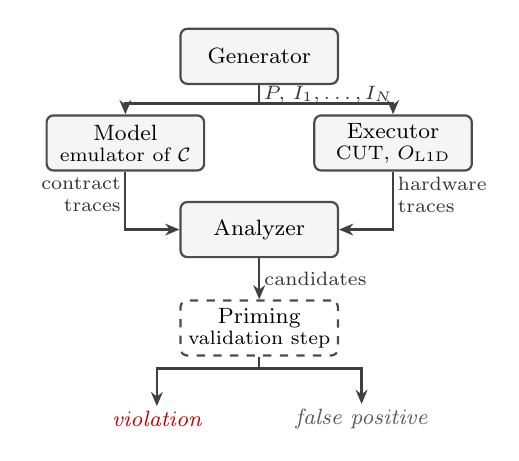
\begin{tikzpicture}[
  font=\footnotesize,
  comp/.style={draw=black!70, fill=black!4, rounded corners=2.5pt, thick,
               align=center, minimum width=20mm, minimum height=7mm,
               inner sep=1.5pt},
  stage/.style={draw=black!70, dashed, fill=white, rounded corners=2.5pt, thick,
                align=center, minimum width=20mm, minimum height=7mm,
                inner sep=1.5pt},
  out/.style={text=#1, font=\footnotesize\itshape, inner sep=1.5pt},
  lbl/.style={font=\scriptsize, text=black!80, inner sep=1.5pt},
  arr/.style={-{Stealth[length=1.8mm,width=1.5mm]}, thick, draw=black!75},
]
  % components
  \node[comp] (gen)   at (0, 0)       {Generator};
  \node[comp] (model) at (-1.7,-1.1) {Model\\[-2pt]{\scriptsize emulator of $\mathcal{C}$}};
  \node[comp] (exec)  at ( 1.7,-1.1) {Executor\\[-2pt]{\scriptsize CUT, $\ol$}};
 
  % analyzer component, then priming as a separate validation step
  \node[comp]  (an)    at (0,-2.2) {Analyzer};
  \node[stage] (prime) at (0,-3.45)  {Priming\\[-2pt]{\scriptsize validation step}};

  \node[out=red!75!black] (viol) at (-1.3,-4.6) {violation};
  \node[out=black!65]    (fp)   at ( 1.3,-4.6) {false positive};
 
  % generator -> model / executor
  \coordinate (split) at (0,-0.6);
  \draw[thick, draw=black!75] (gen.south) -- (split);
  \draw[arr] (split) -| (model.north);
  \draw[arr] (split) -| (exec.north);
  \node[lbl, right] at ($(gen.south)!0.5!(split)$) {$P,\, I_1,\dots,I_N$};
 
  % model / executor -> analyzer
  \draw[arr] (model.south) |- (an.west);
  \draw[arr] (exec.south)  |- (an.east);
  \node[lbl, left, align=right] at ($(model.south)!0.4!(model.south |- an.west)$) {contract\\traces};
  \node[lbl, right, align=left] at ($(exec.south)!0.4!(exec.south |- an.east)$)   {hardware\\traces};
 
  % analyzer -> priming
  \draw[arr] (an) -- node[lbl, right] {candidates} (prime);
 
  % priming -> outcomes
  \coordinate (split2) at ($(prime.south)+(0,-0.15)$);
  \draw[thick, draw=black!75] (prime.south) -- (split2);
  \draw[arr] (split2) -| (viol.north);
  \draw[arr] (split2) -| (fp.north);
 
  % symmetric bounding box, so the Generator is centered
  \path let \p1 = (current bounding box.north east),
            \p2 = (current bounding box.south west),
            \n1 = {max(\x1, -\x2)} in
        coordinate (bbne) at (\n1, \y1) coordinate (bbsw) at (-\n1, \y2);
  \pgfresetboundingbox
  \useasboundingbox (bbsw) rectangle (bbne);
\end{tikzpicture}
\caption{\textsc{Revizor}'s testing pipeline: four components (solid) and
the priming validation step (dashed).}
\label{fig:revizor}
\end{figure}
 
\paragraph{Hardware traces.}
Measuring the full trace is infeasible, so \textsc{Revizor} approximates
Eq.~\eqref{eq:htrace} by measuring only the L1D cache, once the input has finished
executing:
\begin{equation}
\Al(P,I,\mathit{Ctx}) = \ol(\mu_n),
\label{eq:htrace-l1d}
\end{equation}
where $\ol$ yields the L1D lines, or sets, that the execution accessed.
The measurement uses a cache side channel such as Flush+Reload or Prime+Probe and is
repeated to filter noise. \textsc{Revizor} thus tests $\mathcal{C}$ with respect to
$\ol$, and an effect in another structure enters the hardware trace only
once it propagates into the L1D.
 
\paragraph{\uarch context.}
Since a black-box CPU's context cannot be set directly, \textsc{Revizor} sets it indirectly.
It runs the inputs $I_1,\dots,I_N$ back to back, with only a partial reset such as cache
flushes between them~\cite{revizor,hide_seek}, so the context $\mathit{Ctx}_k$ of each input is
the state its predecessors leave behind. This yields contexts that are diverse, which helps
trigger mispredictions, yet deterministic, so replaying it reproduces a measurement.
 
\paragraph{Priming.}
Because each input runs in its own context, a candidate violation is a pair of
contract-equivalent inputs $I_i$ and $I_j$ ($i<j$) whose traces, each in its own
context, differ:
\begin{equation}
\begin{gathered}
\mathcal{C}(P,I_i) = \mathcal{C}(P,I_j) \\
\land\;
\Al(P,I_i,\mathit{Ctx}_i) \neq
\Al(P,I_j,\mathit{Ctx}_j).
\end{gathered}
\label{eq:candidate}
\end{equation}
\noindent Unlike in Eq.~\eqref{eq:violation}, the difference may therefore stem from the
contexts rather than the inputs. Priming~\cite{revizor} closes this gap by re-running the sequence
twice, once with $I_j$ at position $i$ and once with $I_i$ at position~$j$. Because
the inputs preceding each position are unchanged, both inputs are tested in
both contexts. The candidate is classified as a \emph{false positive} if
\begin{equation}
\begin{gathered}
\Al(P,I_i,\mathit{Ctx}_i) =
\Al(P,I_j,\mathit{Ctx}_i) \\
\land\;
\Al(P,I_i,\mathit{Ctx}_j) =
\Al(P,I_j,\mathit{Ctx}_j),
\end{gathered}
\label{eq:priming}
\end{equation}
\noindent and as a violation otherwise. In other words, priming checks whether
the trace difference follows an input's position in the sequence rather than
its content.

\paragraph{Boosting.}
Uniformly random inputs are rarely contract-equivalent. Fewer than $6\%$ are in the
measurements of~\cite{hide_seek}, and none for test cases with at least $16$ memory accesses,
so random sampling almost never yields the equivalent pair a candidate needs.
\textsc{Revizor} therefore \emph{boosts} each input $I$ into further inputs $I',I'',\dots$ of
the same class~\cite{hide_seek}. It runs the contract model on $I$, keeps the parts of the
input that the contract trace depends on, and re-randomizes the rest. Our detection method relies
on these boosted classes (\S\ref{sec:detect}).

%-------------------------------------------------------------------------------
\section{Speculative-exception fuzzing}
\label{sec:precond}
% Preamble: \usepackage{booktabs}
%           \usepackage{tikz}\usetikzlibrary{arrows.meta,calc}
%-------------------------------------------------------------------------------
\begin{table}[!tb]
\centering
\footnotesize
\setlength{\tabcolsep}{2pt}
\caption{Automated transient-leakage testing tools, by methodology class~\cite{arcus_sok}: \emph{MRT}
(model-based relational testing), \emph{OIF} (observation-independent fuzzing), and \emph{RT}
(relational testing). \emph{Faults}: generates architecturally faulting instructions.
\emph{Spec.\ only faults}: generates faults only on a speculative path.}
\label{tab:related}
\begin{tabular}{@{}l l l c c@{}}
\toprule
Tool & Method & Platform & Faults & \makecell{Spec.\\only\\faults} \\
\midrule
\multicolumn{5}{@{}l}{\emph{\uarch, post-silicon}} \\
\textsc{Revizor}, Hide \& Seek~\cite{revizor,hide_seek}       & MRT & x86 CPU & \xmark & \xmark \\
Spec.\ at Fault, Enter/Exit~\cite{speculation_fault,isolation} & MRT & x86 CPU & \cmark & \xmark \\
Scam-V~\cite{scamv}                      & MRT & Arm CPU & \xmark & \xmark \\
Osiris~\cite{osiris}                     & OIF & x86 CPU & \xmark & \xmark \\
Transynther~\cite{transynther}           & OIF & x86 CPU & \cmark & \xmark \\
\midrule
\multicolumn{5}{@{}l}{\emph{Pre-silicon, simulators and RTL designs}} \\
AMuLeT~\cite{amulet}                     & MRT            & x86 gem5   & \xmark & \xmark \\
IntroSpectre~\cite{introspectre}         & OIF            & RISC-V RTL & \cmark & part.$^{\dagger}$ \\
SpecDoctor~\cite{specdoctor}             & RT & RISC-V RTL & \cmark & part.$^{\ddagger}$ \\
\midrule
This work                                & MRT & Arm CPU & \xmark & \cmark \\
\bottomrule
\end{tabular}

\smallskip
\raggedright\footnotesize
$^{\dagger}$Page faults only: a helper gadget can place a page-faulting load behind a mispredicted branch.
$^{\ddagger}$Permission faults on the planted secret only.
\end{table}

For a test case to run to completion, every instruction on its architectural path must satisfy
its operand conditions. For example, each memory access must reach a mapped, canonical address
with the right permissions, and under MTE or Pointer Authentication a pointer must carry the
correct metadata to pass validation. A condition that fails architecturally raises an exception
and ends the run. On a speculative path the same failure never faults architecturally. If the satisfied and the
violated cases then leave distinguishable \uarch traces, an attacker can tell which case occurred, and so learn about the protected operand. Extracting this information without ever faulting the victim is what
gives such leaks practical attack value, and is what PACMAN~\cite{pacman} and TikTag~\cite{tiktag}
exploit (\S\ref{sec:intro}). Existing fuzzers either keep these conditions satisfied
by construction, or violate them architecturally and fault, so neither produces a condition that
fails only speculatively (Table~\ref{tab:related}).

Our goal is a single program that stays architecturally correct for every random input, yet
violates these conditions on speculative paths alone, so no violation ever retires. The difficulty
is that whether an instruction is reached, and with which operand, depends on the program's path
conditions, which are costly to solve even for small programs. Scam-V spends a few seconds
generating each input pair~\cite{scamv_micro}, and symbolic input generation is about two orders of magnitude
slower than dependency tracking~\cite{hide_seek}. We sidestep this solving with a layer of indirection: each instruction we fuzz reads its operand
from a \emph{global value table} (GVT), so filling the GVT decides what each reads. Because the
correct value can depend on runtime state, such as the system state or previously executed
instructions, we obtain it with a single run per input under a lightweight architectural debugger
(\S\ref{sec:port}) (Figure~\ref{fig:flow}).

\begin{figure}[t]
\centering
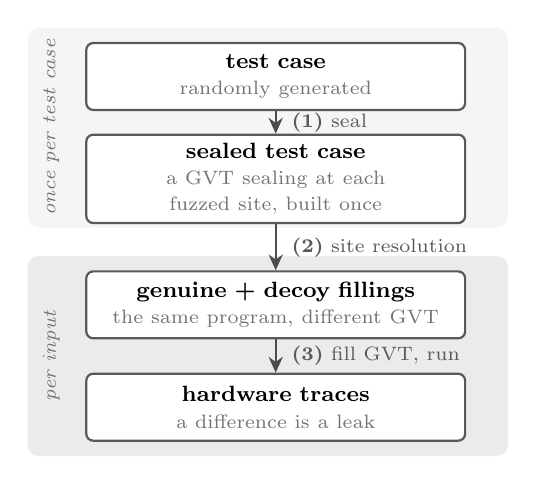
\begin{tikzpicture}[
  font=\footnotesize,
  stage/.style={draw=black!65, fill=white, rounded corners=2.5pt, thick,
                align=center, text width=46mm, minimum height=8.5mm, inner sep=3pt},
  ar/.style={-{Stealth[length=2mm,width=1.8mm]}, thick, draw=black!70},
  al/.style={font=\scriptsize, text=black!65, anchor=west},
  pl/.style={font=\scriptsize\itshape, text=black!55, rotate=90},
]
  \def\gy{1.3}
  \def\dg{0.3}
  \fill[black!4, rounded corners=4pt] (-3.15,0.62) rectangle (2.95,-\gy-0.62);
  \fill[black!8, rounded corners=4pt] (-3.15,-2*\gy+0.62-\dg) rectangle (2.95,-3*\gy-0.62-\dg);
  \node[stage] (a) at (0,0)       {\textbf{test case} \\ {\scriptsize\color{black!55} randomly generated}};
  \node[stage] (b) at (0,-\gy)    {\textbf{sealed test case} \\ {\scriptsize\color{black!55} a GVT sealing at each fuzzed site, built once}};
  \node[stage] (d) at (0,-2*\gy-\dg)  {\textbf{genuine + decoy fillings} \\ {\scriptsize\color{black!55} the same program, different GVT}};
  \node[stage] (e) at (0,-3*\gy-\dg)  {\textbf{hardware traces} \\ {\scriptsize\color{black!55} a difference is a leak}};
  \draw[ar] (a) -- (b) node[al,midway,xshift=2pt]{\textbf{(1)}~seal};
  \draw[ar] (b) -- (d) node[al,midway,xshift=2pt]{\textbf{(2)}~site resolution};
  \draw[ar] (d) -- (e) node[al,midway,xshift=2pt]{\textbf{(3)}~fill GVT, run};
  \node[pl] at (-2.85,-0.5*\gy)     {once per test case};
  \node[pl] at (-2.85,-2.5*\gy-\dg) {per input};
\end{tikzpicture}
\caption{The speculative-exception-fuzzing pipeline. The program is sealed once and stays
byte-identical across fillings.}
\label{fig:flow}
\end{figure}

\paragraph{The global value table.}
We call each instruction whose operands we fuzz a \emph{site}. The GVT holds the value each site
reads at run time, and mirrors the global offset table of dynamic linking: the indexes are fixed
when the program is built, while the values are filled per input, just before execution. Because a
site reads some of its operands from the GVT, we can inject violating values at a site directly,
without rewriting the program or searching for an input whose data flow produces them. The GVT
entries thus decide which sites are violated. The table is part of the input, so two inputs that
differ only in their GVT are different inputs. We keep the GVT in registers rather than in memory,
so a lookup is not a memory access and adds no long-latency operation that could perturb the
\uarch we measure. Specifically, we use the Advanced SIMD vector registers,\footnote{\texttt{FEAT\_AdvSIMD}.}
which offer far more capacity than the general-purpose ones.

\paragraph{Genuine and decoy fillings.}
A run of the program is fixed by how we fill the GVT. The \emph{genuine} filling gives every site
its correct value, the one the architectural flow expects. A \emph{decoy} filling instead forges
the value (a wrong PAC, a mismatched tag, or a non-canonical address) at a random subset of the
sites reached only speculatively, and keeps the correct value everywhere a site retires.
Table~\ref{tab:sealings} lists the sealing primitives with their genuine and decoy values.

\begin{table}[t]
\centering
\footnotesize
\setlength{\tabcolsep}{4pt}
\caption{Sealing primitives.}
\label{tab:sealings}
\begin{tabular}{@{}l l l@{}}
\toprule
Condition & genuine value & decoy value \\
\midrule
PAC signature          & correct signature & forged signature \\
MTE tag                & matching tag      & mismatched tag \\
Canonicality           & canonical address & non-canonical address \\
Sign-extension         & correct sign bit  & flipped sign bit \\
Indirect branch target & valid target      & non-canonical / misaligned target \\
\bottomrule
\end{tabular}
\end{table}

\paragraph{Sealing a site.}
We call the instrumentation at one fuzzed site a \emph{sealing}. The generator walks the test
case statically and inserts a sealing before each instruction of interest
(Figure~\ref{fig:precond-seal}). It consists of a \texttt{UMOV}, which copies the site's GVT value
from its vector element into a general-purpose register, followed by the data-processing
instructions that apply it. For example, a PAC or an MTE tag is read from the GVT and inserted
into the relevant field of the pointer with \texttt{BFI}.

\begin{figure*}[t]
\centering
\footnotesize
\begin{minipage}[t]{0.46\linewidth}
\centering\textbf{A \texttt{PAC} sealing}\par\smallskip
\begin{verbatim}
UMOV  wT, GVT.h[i]   // read signature
BFI   x0, xT, PAC    // into PAC field
AUTDA x0, x1         // authenticate x0
LDR   x2, [x0]       // guarded access
\end{verbatim}
\vspace{\baselineskip}
\raggedright\small
\emph{genuine} fill: the correct signature.\par
\emph{decoy} fill: a forged signature.
\end{minipage}\hfill
\begin{minipage}[t]{0.46\linewidth}
\centering\textbf{An \texttt{MTE} sealing}\par\smallskip
\begin{verbatim}
UMOV  wT, GVT.b[i]   // read tag
BFI   x0, xT, #56,#4 // into tag field
LDR   x2, [x0]       // tag-checked access
UMOV  wT, GVT.b[j]   // read cell tag
BFI   x0, xT, #56,#4 // retag back
\end{verbatim}
\raggedright\small
\emph{genuine} fill: the matching cell tag.\par
\emph{decoy} fill: a mismatched tag.\par
The second \texttt{BFI} always restores \texttt{x0} to the genuine tag.
\end{minipage}
\caption{A \texttt{PAC} sealing and an \texttt{MTE} sealing. The slot is fixed and identical
in every filling, and only the GVT value differs between the genuine and decoy fillings.
The \texttt{MTE} sealing restores the genuine tag with a second \texttt{BFI} after the access.}
\label{fig:precond-seal}
\end{figure*}

\paragraph{Site resolution.}
When we build the program, each site's genuine value is often unknown, such as the PAC of a
pointer the input computes or the Allocation Tag of the granule it reaches, and so is whether the
architectural flow reaches the site at all. \emph{Site resolution} settles both in one run of a
lightweight architectural debugger (the contract executor, described in \S\ref{sec:port}) over an
initially empty GVT, the \emph{resolution trace}. Each time the run reaches a site whose genuine
value depends on the live state, a small routine computes that value and writes it into the site's
GVT entry, much as a dynamic linker fills a symbol's entry on first use. At a PAC site, for
example, it computes the PAC of the pointer the \texttt{AUT*} is about to authenticate, and at an
MTE site it reads the Allocation Tag of the accessed granule. Because the resolution run executes
the genuine instructions, it doubles as the genuine contract trace, and its speculation stack
(described in \S\ref{sec:port}) records the depth at which each site is reached, marking those
never reached architecturally as decoy-eligible.

\paragraph{Confining a condition violation.}
We want to compare contract-equivalent inputs under both the genuine and decoy fillings, so the
two must produce an identical contract trace even though the decoy injects a violating value
through the GVT (Eq.~\eqref{eq:violation}). We therefore confine the decoy value to the sealed
access and keep it from reaching the contract trace: immediately after the access we overwrite any
injected value with a consistent value for both fillings. Some instructions, such as \texttt{AUT*},
do this for free: \texttt{AUT*} overwrites the signature by sign-extending from bit~55, which is
kept identical under both fillings. Others, such as memory accesses and indirect branches, require
an explicit overwrite. A load, for example, does not overwrite the tag or canonicality bits it
checks, so the pointer keeps the decoy value past the access, and we restore it to the genuine
value, retagging with the correct tag for \texttt{MTE} and undoing the mask for canonicality.

\paragraph{Generating same-contract inputs.}
To compare an input against contract-equivalent ones, we generate further inputs of its contract
class in two modes, \emph{contract-driven} and \emph{strict}. Contract-driven uses boosting~\cite{hide_seek}
to draw a new input from the class, varying the GVT entries the contract leaves untainted. Strict
instead holds the entire input byte-identical across the two runs and varies only the GVT, targeting
speculative exceptions alone.
\paragraph{Widening the speculative window.}
A sealed access leaves a \uarch trace only if it executes before the speculative window closes, and
a random test case does not control that window's length. To give the access enough time, we attach
a \emph{template} that holds the window open (Figure~\ref{fig:tiktag-tmpl}): eight dependent
\texttt{SDIV} instructions delay the guarding \texttt{CBNZ}, so its not-taken shadow speculates for
the chain's length, while an \texttt{ORR} keeps the branch architecturally taken. A long speculation
window proved necessary for TikTag: without the template the campaign never surfaced the leak,
whereas with it TikTag appeared and was verified after $8$ test cases, in about $2$ minutes.

%-------------------------------------------------------------------------------
\section{Source-Agnostic Violation Detection}
\label{sec:detect}
\providecommand{\Al}{\mathit{Attack}_{\mathrm{L1D}}}
\providecommand{\IS}{\mathrm{IS}}
\providecommand{\run}{\mathit{run}}

Throughout this section we fix an observer $\obs$, the structure the attacker monitors~\cite{contracts}.
We show that priming~\cite{revizor}, the validation step that turns candidates into reported
violations, has a structural blind spot. A leak can be real and lie within a natural extension of
\textsc{Revizor}'s threat model, yet be discarded on every run. This happens when the leaking input first perturbs a
structure other than $\obs$, a transmitting structure, and that effect reaches $\obs$ only in a later run,
possibly after passing through a series of transmitting structures. We characterize this class,
prove that priming never reports it, and give a detection method that reports it while reading only
$\obs$. It thus detects a leak that reaches $\obs$ from another structure, even one not publicly known to
exist, while monitoring only $\obs$.

We instantiate $\obs$ as the L1D cache. Its state can be measured on almost any CPU through
well-studied cache side channels. Observing further structures would define a different threat
model, and would work only for structures that are known and measurable. Our method is
\emph{source-agnostic} and complements such extensions.

Our extension to the threat model is a practical attacker that runs a fixed follow-up program before
it reads $\obs$. We extend the contract-violation definition to it, show that our method widens what
fuzzing can detect, recovering a subset of the violations priming discards,\footnote{It does not
subsume priming: with lanes we give up the within-lane comparisons priming makes, discussed in
\S\ref{sec:detect-priming}.} and give two localizers that pinpoint the responsible input pair.

%===============================================================================
\subsection{Notation and assumptions}
\label{sec:detect-model}
%===============================================================================

Write $\run(P,I,\mu)$ for the \uarch state left by executing $P$ on input $I$
from state $\mu$. A \emph{batch} is a sequence of inputs that the executor runs back to back.

\begin{assumption}[High-quality initialization]
\label{asm:is}
Every batch opens with the same \emph{initialization sequence} $\IS$, a high-quality reset that
brings the core to the same state $\mu_\IS$, independent of the state before it.
\end{assumption}

\noindent For example, $\IS$ clears the branch history with the taken-branch loop Arm recommends
against Spectre-BHB~\cite{arm_spectre_bhb}. A black-box core cannot be reset
perfectly~\cite{hide_seek}, so $\IS$ is best-effort and residual state it leaves can cause false
positives.

\begin{assumption}[Priming]
\label{asm:prime}
As in \textsc{Revizor}~\cite{revizor}, execution of one input sets the microarchitectural context for
the next, so the inputs before a given input determine the context it runs from, deterministically
enough for the trace comparisons.
\end{assumption}

We write $\batch{I_0,\dots,I_n}$ for the batch that runs $\IS$ and then the inputs
$I_0,\dots,I_n$, so the first input starts from approximately $\mu_\IS$. Each reading repeats the
batch and aggregates the repetitions, as \textsc{Revizor} does to filter noise~\cite{revizor}. Thus two
readings differ only when the underlying trace distributions differ, not through noise. The method
and its soundness below are stated for an arbitrary observer $\obs$. Our implementation instantiates
$\obs$ as the L1D cache, so the L1D trace of Eq.~\eqref{eq:htrace-l1d} is
$\Al(P,I,\mathit{Ctx})=\ol(\run(P,I,\mathit{Ctx}))$.

%===============================================================================
\begin{figure*}[t]
\centering
\begin{minipage}[t]{0.48\textwidth}
\centering
\caption{A BTB leak current priming discards. A later input's speculative call to the carried
target reveals the target an earlier input supplied.}
\label{fig:miss}
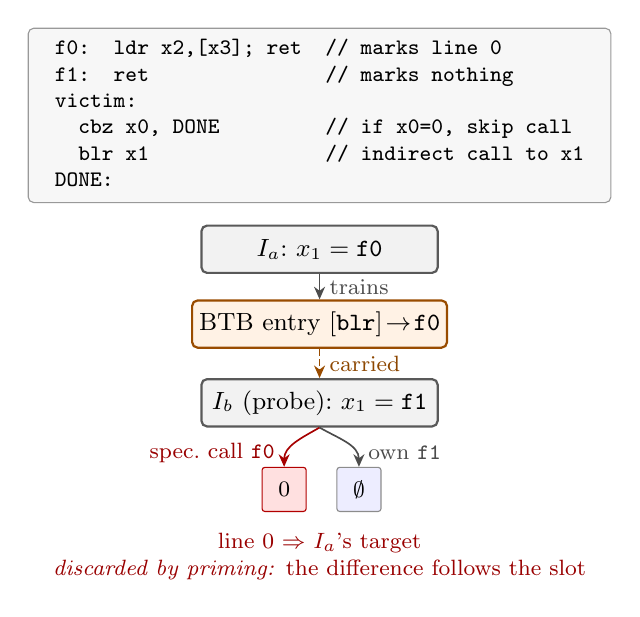
\begin{tikzpicture}[
  font=\small,
  box/.style={draw=black!65, fill=black!5, rounded corners=2pt, thick, align=center,
              inner sep=2.5pt, minimum width=30mm, minimum height=6mm},
  carr/.style={draw=orange!60!black, fill=orange!10, rounded corners=2pt, thick,
               align=center, inner sep=2.5pt, minimum width=30mm, minimum height=6mm},
  code/.style={draw=black!40, fill=black!3, rounded corners=2pt, align=left,
               inner sep=3pt, font=\ttfamily\footnotesize, minimum width=74mm},
  cell/.style={draw=black!45, rounded corners=1pt, minimum width=5.6mm,
               minimum height=5.6mm, inner sep=0pt, font=\footnotesize},
  hot/.style={cell, draw=red!70!black, fill=red!12},
  cold/.style={cell, fill=blue!7},
  arr/.style={-{Stealth[length=1.6mm,width=1.4mm]}, semithick, draw=black!70},
  rarr/.style={-{Stealth[length=1.6mm,width=1.4mm]}, semithick, draw=red!65!black},
  darr/.style={-{Stealth[length=1.6mm,width=1.4mm]}, semithick, draw=orange!60!black, dash pattern=on 2.5pt off 1.2pt},
  lbl/.style={font=\footnotesize, text=black!70, align=center},
  rlbl/.style={font=\footnotesize, text=red!60!black, align=center},
  drop/.style={font=\footnotesize, text=red!60!black, align=center},
]
  \node[code] at (0,3.25) {\begin{tabular}{@{}l@{\ \ }l@{}}
    f0: ldr x2,[x3]; ret & // marks line 0\\
    f1: ret & // marks nothing\\
    victim: & \\
    \ \ cbz x0, DONE & // if x0=0, skip call\\
    \ \ blr x1 & // indirect call to x1\\
    DONE: & \\
  \end{tabular}};
  \node[box]  (a1) at (0,1.55) {$I_a$:\ $x_1=\texttt{f0}$};
  \node[carr] (ac) at (0,0.6)  {BTB entry $[\texttt{blr}]\!\to\!\texttt{f0}$};
  \node[box]  (a2) at (0,-0.4) {$I_b$ (probe):\ $x_1=\texttt{f1}$};
  \draw[arr]  (a1) -- node[lbl,right]{trains} (ac);
  \draw[darr] (ac) -- node[lbl,right,text=orange!55!black]{carried} (a2);
  \node[hot]  (as0) at (-0.45,-1.5) {$0$};
  \node[cold] (as1) at ( 0.5,-1.5) {$\emptyset$};
  \draw[rarr] (a2.south) to[out=-150,in=90] node[rlbl,left,pos=0.9,yshift=3pt]{spec.\ call \texttt{f0}} (as0.north);
  \draw[arr]  (a2.south) to[out=-30,in=90]  node[lbl,right,pos=0.9,yshift=3pt]{own \texttt{f1}} (as1.north);
  \node[drop] at (0,-2.35) {line $0$ $\Rightarrow$ $I_a$'s target\\\emph{discarded by priming:} the difference follows the slot};
\end{tikzpicture}
\end{minipage}\hfill
\begin{minipage}[t]{0.48\textwidth}
\centering
\caption{A prefetcher leak current priming discards. A later input's carried prefetch stream
reveals an earlier input's stride.}
\label{fig:miss-pf}
\vspace{12pt}
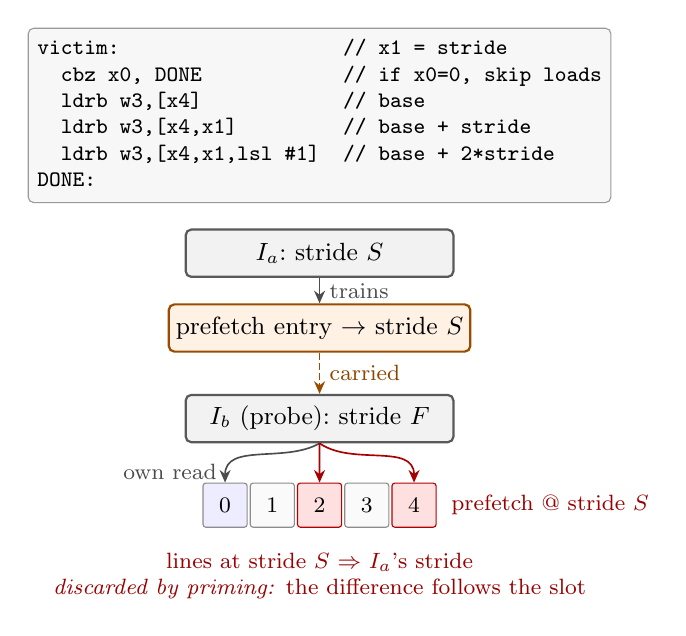
\begin{tikzpicture}[
  font=\small,
  box/.style={draw=black!65, fill=black!5, rounded corners=2pt, thick, align=center,
              inner sep=2.5pt, minimum width=34mm, minimum height=6mm},
  carr/.style={draw=orange!60!black, fill=orange!10, rounded corners=2pt, thick,
               align=center, inner sep=2.5pt, minimum width=34mm, minimum height=6mm},
  code/.style={draw=black!40, fill=black!3, rounded corners=2pt, align=left,
               inner sep=3pt, font=\ttfamily\footnotesize, minimum width=74mm},
  cell/.style={draw=black!45, rounded corners=1pt, minimum width=5.6mm,
               minimum height=5.6mm, inner sep=0pt, font=\footnotesize},
  hot/.style={cell, draw=red!70!black, fill=red!12},
  cold/.style={cell, fill=blue!7},
  none/.style={cell, fill=black!2},
  arr/.style={-{Stealth[length=1.6mm,width=1.4mm]}, semithick, draw=black!70},
  rarr/.style={-{Stealth[length=1.6mm,width=1.4mm]}, semithick, draw=red!65!black},
  darr/.style={-{Stealth[length=1.6mm,width=1.4mm]}, semithick, draw=orange!60!black, dash pattern=on 2.5pt off 1.2pt},
  lbl/.style={font=\footnotesize, text=black!70, align=center},
  rlbl/.style={font=\footnotesize, text=red!60!black, align=center},
  drop/.style={font=\footnotesize, text=red!60!black, align=center},
]
\def\bx{0}
\node[code] at (\bx,3.3) {\begin{tabular}{@{}l@{\ \ }l@{}}
  victim: & // x1 = stride\\
  \ \ cbz x0, DONE & // if x0=0, skip loads\\
  \ \ ldrb w3,[x4] & // base\\
  \ \ ldrb w3,[x4,x1] & // base + stride\\
  \ \ ldrb w3,[x4,x1,lsl \#1] & // base + 2*stride\\
  DONE: & \\
\end{tabular}};
\node[box]  (b1) at (\bx,1.55) {$I_a$:\ stride $S$};
\node[carr] (bc) at (\bx,0.6)  {prefetch entry $\to$ stride $S$};
\node[box]  (b2) at (\bx,-0.55) {$I_b$ (probe):\ stride $F$};
\draw[arr]  (b1) -- node[lbl,right]{trains} (bc);
\draw[darr] (bc) -- node[lbl,right,text=orange!55!black]{carried} (b2);
\foreach \i in {0,...,4}{
  \ifnum\i=0 \node[cold] (bs\i) at ({\bx-1.2+\i*0.6},-1.65) {\i};\else
  \ifnum\i=2 \node[hot]  (bs\i) at ({\bx-1.2+\i*0.6},-1.65) {\i};\else
  \ifnum\i=4 \node[hot]  (bs\i) at ({\bx-1.2+\i*0.6},-1.65) {\i};\else
  \node[none] (bs\i) at ({\bx-1.2+\i*0.6},-1.65) {\i};\fi\fi\fi}
\draw[arr]  (b2.south) to[out=-150,in=90] node[lbl,left,pos=0.9]{own read} (bs0.north);
\draw[rarr] (b2.south) to[out=-90,in=90]  (bs2.north);
\draw[rarr] (b2.south) to[out=-35,in=90]  (bs4.north);
\node[rlbl, anchor=west] at ({\bx+1.55},-1.65) {prefetch @ stride $S$};
\node[drop] at (\bx,-2.55) {lines at stride $S$ $\Rightarrow$ $I_a$'s stride\\\emph{discarded by priming:} the difference follows the slot};
\end{tikzpicture}
\end{minipage}

\vspace{8pt}
\begin{minipage}[t]{0.48\textwidth}
\centering
\footnotesize
\setlength{\tabcolsep}{7pt}
\begin{tabular}{@{}lcc}
\toprule
 & \begin{tabular}[b]{@{}c@{}}slot after\\$I_a$ (\texttt{f0})\end{tabular} & \begin{tabular}[b]{@{}c@{}}slot after\\$I_b$ (\texttt{f1})\end{tabular} \\
\midrule
$I_b$ (\texttt{f1}) & \cellcolor{blue!8}$\{0\}^\star$ & \cellcolor{green!9}$\emptyset$ \\
$I_c$ (\texttt{f1}) & \cellcolor{blue!8}$\{0\}$ & \cellcolor{green!9}$\emptyset^\star$ \\
\midrule
\textit{\footnotesize priming compares} & \cellcolor{blue!8}equal & \cellcolor{green!9}equal \\
\bottomrule
\end{tabular}
\captionof{table}{Priming the candidate $(I_b,I_c)$ of Figure~\ref{fig:miss}. Line $0$ is\protect\newline the target carried from $I_a$. Starred cells flagged it.\protect\newline Both columns agree, so priming
discards it as a false positive.}
\label{tab:prime-drop}
\end{minipage}\hfill
\begin{minipage}[t]{0.48\textwidth}
\centering
\footnotesize
\setlength{\tabcolsep}{7pt}
\begin{tabular}{@{}lcc}
\toprule
 & \begin{tabular}[b]{@{}c@{}}slot after\\$I_a$ (stride $S$)\end{tabular} & \begin{tabular}[b]{@{}c@{}}slot after\\$I_b$ (stride $F$)\end{tabular} \\
\midrule
$I_b$ (stride $F$) & \cellcolor{blue!8}$\{0,F,2F,S,2S\}^\star$ & \cellcolor{green!9}$\{0,F,2F\}$ \\
$I_c$ (stride $F$) & \cellcolor{blue!8}$\{0,F,2F,S,2S\}$ & \cellcolor{green!9}$\{0,F,2F\}^\star$ \\
\midrule
\textit{\footnotesize priming compares} & \cellcolor{blue!8}equal & \cellcolor{green!9}equal \\
\bottomrule
\end{tabular}
\captionof{table}{Priming the candidate $(I_b,I_c)$ of Figure~\ref{fig:miss-pf}.
$\{S,2S\}$ are the stale prefetches carried from $I_a$. Starred cells flagged it. Both
columns agree, so priming discards it as a false positive.}
\label{tab:prime-drop-pf}
\end{minipage}
\end{figure*}

\subsection{Leaks priming discards}
\label{sec:detect-gap}
%===============================================================================

We make the blind spot concrete with two examples, one leaking through the branch target buffer and
one through a data prefetcher. In each, a secret that an earlier input leaves in that structure
reaches a later run's L1D, so the leak is real, yet priming discards the pair. We close with the
formal proof.

\paragraph{A BTB leak.}
Consider the gadget in Figure~\ref{fig:miss}. Every input sets \texttt{x0} to zero, so the guard
\texttt{cbz x0, DONE} is taken and \texttt{blr x1} is skipped. The call runs only when the guard is
mispredicted, on the transient path. It never retires, so \texttt{x1} never enters the contract
trace. Under \textsc{CT-SEQ} every input then shares one class, whatever target it carries. One
target, \texttt{f0}, loads line~$0$. The other, \texttt{f1}, touches nothing.

The call site's indirect predictor still learns each run's target from the speculative execution
and keeps it for the next. The target one input supplies therefore surfaces only on a later run at
the same site, which speculatively calls the carried target and pulls its line into the L1D. The
BTB entry acts as the transmitting structure, and the observation medium is the L1D.



\paragraph{Priming drops it.}
Take $\batch{I_a,I_b,I_c}$ with $x_1=\texttt{f0}$ for $I_a$ and $x_1=\texttt{f1}$ for $I_b$ and
$I_c$. All three share a class, since \texttt{x1} is invisible to the CT-SEQ contract. Assuming the
initialization sequence leaves the BTB entry empty, $I_a$ touches nothing in memory and
trains the entry to \texttt{f0}. $I_b$ then inherits \texttt{f0}, speculatively calls it, and leaves
$\{0\}$, while $I_c$ inherits \texttt{f1} from $I_b$ and leaves $\emptyset$. The differing footprints flag
$(I_b,I_c)$ by Eq.~\eqref{eq:candidate}. The difference comes from the carried BTB target, not from
the two inputs. In a matched slot they leave the same footprint (Table~\ref{tab:prime-drop}).
Priming compares them slot by slot, finds agreement, and discards the pair as a false positive
(Eq.~\eqref{eq:priming}), even though $I_a$'s target reached the probe's L1D.





\paragraph{A prefetcher leak.}
The gadget in Figure~\ref{fig:miss-pf} reads \texttt{base[0]}, \texttt{base[s]}, and
\texttt{base[2s]} at a stride~$s$ the input chooses, behind the same guard, so the loads run only
speculatively and \texttt{s} never enters the CT-SEQ contract trace. They still train a data prefetcher
that locks onto a constant stride and runs ahead. After
one input trains stride~$S$, a later same-class input reads at a fixed stride~$F$, yet the carried
stream keeps prefetching at~$S$ and pulls in lines the input never requests, so its L1D footprint
reveals the earlier stride. The prefetch entry acts as the transmitting structure, and the observation medium is again
the L1D.

\paragraph{Priming drops it too.}
Take $\batch{I_a,I_b,I_c}$ with $I_a$ at stride~$S$ and $I_b,I_c$ at a fixed stride~$F$ over the
same base. All three share a class, since the stride is invisible to the CT-SEQ contract. Assuming
the initialization sequence leaves the prefetch entry empty, $I_a$ runs at stride~$S$ and trains
the entry to that stride. $I_b$
inherits it, so the carried stride-$S$ stream adds the stale lines $\{S,2S\}$ to its own
$\{0,F,2F\}$, while $I_c$ inherits $I_b$'s stride~$F$ and leaves only $\{0,F,2F\}$. The differing
footprints flag $(I_b,I_c)$ by Eq.~\eqref{eq:candidate}. The difference comes from the carried
prefetch stream, not from the two inputs. In a matched slot they leave the same footprint
(Table~\ref{tab:prime-drop-pf}). Priming compares them slot by slot, finds agreement, and discards
the pair as a false positive (Eq.~\eqref{eq:priming}), even though $I_a$'s stride reached the
probe's L1D.



\paragraph{The general pattern.}
In both examples the flagged pair is indistinguishable from any common starting state, and what
flags it is written by an earlier input and carried into a later run. The gadget below shows this in
the abstract: it loads a carried bit $s$, then overwrites $s$ with an input-dependent bit
$g(\mathrm{input})$ the contract does not expose.

{\footnotesize
\begin{verbatim}
// s: one bit of a uarch structure, unseen by C.
victim(input):
    load A[s]       // footprint = line s
    s := g(input)   // write s, hidden from C
\end{verbatim}
}

\begin{proposition}[Priming's blind spot]
\label{prop:priming-blind}
Assuming $\IS$ clears $s$ to $0$ (Assumption~\ref{asm:is}) and a non-constant $g$, there are two
contract-equivalent inputs whose flagged candidate priming discards, even though the trace reveals
the value $g$ the earlier input wrote.
\end{proposition}
\begin{proof}
As $g$ is non-constant, pick inputs with $g(I_0)=1$ and $g(I_1)=0$. The contract does not expose the write, so
$\mathcal{C}(P,I_0)=\mathcal{C}(P,I_1)$. In $\batch{I_0,I_1}$, $I_0$ loads line $0$ and sets $s=1$,
then $I_1$ loads line $1$ from that propagated $s$. The footprints differ, so fuzzing flags
$(I_0,I_1)$. Priming reruns each input where the other ran. In $\batch{I_1}$, $I_1$ reveals line $0$,
as $I_0$ did. In $\batch{I_0,I_0}$, the second $I_0$ reveals line $1$, as $I_1$ did. Both match, so
priming discards the pair. Yet an attacker reading $I_1$'s trace learns $g(I_0)$, a secret the
contract hides.
\end{proof}

\noindent Priming's slot-by-slot comparison cancels the carried state of every \uarch structure,
erasing any leakage that reached it from an earlier input.

%===============================================================================
\subsection{Extended contract violations}
\label{sec:detect-observable}
%===============================================================================

An attacker is not limited to reading the L1D when the victim's run ends. It can first run a fixed
follow-up program that brings the carried effect into the L1D. We extend the contract-violation definition
for this attacker.

\begin{definition}[$Q$-hardware trace]
\label{def:qhtrace}
For a program $P$, input $I$, context $\mathit{Ctx}$, observer $\obs$, and a follow-up program $Q$
that takes no input ($\bot$),
\begin{equation}
\mathit{HTrace}^Q = \AQ{\obs}(P,I,\mathit{Ctx}) = \obs\big(\run(Q,\bot,\run(P,I,\mathit{Ctx}))\big).
\end{equation}
\end{definition}

\begin{definition}[Extended contract violation]
\label{def:extviolation}
A tuple $(P,I_1,I_2,\mathit{Ctx},Q)$ violates contract $\mathcal{C}$ with respect to
observer $\obs$ if $\mathcal{C}(P,I_1)=\mathcal{C}(P,I_2)$ and
$\AQ{\obs}(P,I_1,\mathit{Ctx})\neq\AQ{\obs}(P,I_2,\mathit{Ctx})$.
\end{definition}

An empty $Q$ recovers the original contract violation of Eq.~\eqref{eq:violation}. A non-empty
$Q$ covers a leak that surfaces only after further execution, as in Figure~\ref{fig:miss}. Either
way the leak is real. Since $Q$ is fixed and takes no input, a difference in $\obs$ can only come
from which input the victim ran, and the attacker learns it by running $Q$ and reading $\obs$.

The definition allows any follow-up program. Our detector picks a natural one: the same test case
$P$, run on more random inputs that are fixed once chosen. We prove below that every
violation it reports is a genuine extended violation.

%===============================================================================
\subsection{Detecting extended violations with lanes}
\label{sec:detect-construction}
%===============================================================================

To realize this follow-up, we change how \textsc{Revizor} arranges its inputs. Instead of one
flat sequence, we build \emph{lanes}.

\begin{definition}[Lane and lane boosting]
\label{def:lane}
A \emph{lane} is a sequence of $k+1$ inputs
$\lane{\ell}=(\inp{0}{\ell},\dots,\inp{k}{\ell})$, run as the batch $\batch{\lane{\ell}}$.
The first lane, $\lane{a}$, is generated randomly. Each further lane $\lane{b}$ is
derived by \emph{boosting} every entry of $\lane{a}$ (\S\ref{sec:background-revizor}), so $\inp{m}{a}$
and $\inp{m}{b}$ are distinct same-class inputs. Lanes form a matrix: rows are lanes,
column $m$ is one contract class (Figure~\ref{fig:lanes}).
\end{definition}

Because each column is one class, the detector flags a candidate (Eq.~\eqref{eq:candidate}) when
two lanes, say $\lane{a}$ and $\lane{b}$, differ in their L1D trace at the same column. Without
loss of generality, this is the last column, $k$. A candidate violation at an earlier column $\dprobe<k$
cannot depend on later columns, whose inputs run only after it, so dropping them makes $\dprobe$
last. We call column $k$ the \emph{probe}.

\begin{figure}[t]
\centering
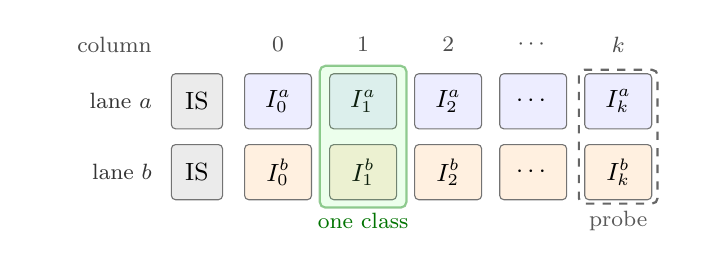
\begin{tikzpicture}[
  font=\small,
  cell/.style={draw=black!55, rounded corners=1.5pt, minimum width=8.5mm,
               minimum height=7mm, inner sep=1pt, align=center},
  acell/.style={cell, fill=blue!7},
  bcell/.style={cell, fill=orange!12},
  is/.style={cell, fill=black!8, minimum width=6.5mm},
  hdr/.style={font=\footnotesize, text=black!70},
  rl/.style={font=\footnotesize, text=black!80, anchor=east},
]
  \def\dx{1.08}
  \def\ya{0} \def\yb{-0.9}
  \path (-1.6,0) -- ({0.5+5*\dx+0.85},0);
  \foreach \i/\lab in {1/0,2/1,3/2,4/$\cdots$,5/$k$}
    \node[hdr] at ({0.5+\i*\dx},0.72) {\lab};
  \node[hdr, anchor=east] at (0.1,0.72) {column};
  \node[rl] at (0.1,\ya) {lane $a$};
  \node[is] at (0.55,\ya) {$\IS$};
  \foreach \i/\lab in {1/$I_0^{a}$,2/$I_1^{a}$,3/$I_2^{a}$,4/$\cdots$,5/$I_k^{a}$}
     \node[acell] at ({0.5+\i*\dx},\ya) {\lab};
  \node[rl] at (0.1,\yb) {lane $b$};
  \node[is] at (0.55,\yb) {$\IS$};
  \foreach \i/\lab in {1/$I_0^{b}$,2/$I_1^{b}$,3/$I_2^{b}$,4/$\cdots$,5/$I_k^{b}$}
     \node[bcell] at ({0.5+\i*\dx},\yb) {\lab};
  \fill[green!60, fill opacity=0.12, rounded corners=2pt]
      ({0.5+2*\dx-0.55},{\ya+0.45}) rectangle ({0.5+2*\dx+0.55},{\yb-0.45});
  \draw[green!50!black, opacity=0.42, thick, rounded corners=2pt]
      ({0.5+2*\dx-0.55},{\ya+0.45}) rectangle ({0.5+2*\dx+0.55},{\yb-0.45});
  \node[hdr, text=green!45!black] at ({0.5+2*\dx},{\yb-0.62}) {one class};
  \draw[black!60, thick, dashed, rounded corners=2pt]
      ({0.5+5*\dx-0.5},{\ya+0.4}) rectangle ({0.5+5*\dx+0.5},{\yb-0.4});
  \node[hdr, text=black!65] at ({0.5+5*\dx},{\yb-0.62}) {probe};
\end{tikzpicture}
\caption{Lanes and classes. Each column is one contract class, and the probe
(column $k$) is where the leak is read.}
\label{fig:lanes}
\end{figure}

\begin{definition}[Splice]
\label{def:splice}
For lanes $\lane{a},\lane{b}$ and a split $t\in\{0,\dots,k+1\}$, the \emph{splice} $\spl{t}$ takes the
columns before $t$ from $\lane{a}$ and the rest from $\lane{b}$,
\begin{equation}
\spl{t}=\big(
  \underbrace{\inp{0}{a},\dots,\inp{t-1}{a}}_{\text{prefix: lane }a},\;
  \underbrace{\inp{t}{b},\dots,\inp{k}{b}}_{\text{suffix: lane }b}\big),
\label{eq:splice}
\end{equation}
which runs as the batch $\batch{\spl{t}}$. The endpoints recover the lanes, $\spl{0}=\lane{b}$ and
$\spl{k+1}=\lane{a}$. Neighboring splices $\spl{t}$ and $\spl{t+1}$ differ only at column $t$, sharing
$\IS$ and every other column (Figure~\ref{fig:boundary}).
\end{definition}

\begin{definition}[Splice measurement]
\label{def:measure}
To measure the splice at $t$, run $\batch{\spl{t}}$ and read the trace of its probe under the observer
$\obs$, the probe being the last input, which is $c_t=\inp{k}{b}$ for $t\le k$ and $c_t=\inp{k}{a}$ for $t=k+1$:
\begin{equation}
r(t)=\At{\obs}(P,\,c_t,\,\mu_t),
\label{eq:rt}
\end{equation}
where $\mu_t$ is the context the preceding inputs leave. Our detector uses $\obs=\ol$.
\end{definition}

The endpoints $r(0)$ and $r(k+1)$ are the probe readings of $\lane{b}$ and $\lane{a}$, the two lanes
that flagged the candidate, so $r(0)\neq r(k+1)$.

%===============================================================================
\subsection{Boundaries and what they guarantee}
\label{sec:detect-soundness}
%===============================================================================

A \emph{boundary} is a split $t$ with $r(t)\neq r(t+1)$.

\textbf{A boundary always exists.} Since $r(0)\neq r(k+1)$, the readings cannot all be equal, so
some neighboring pair differs, and some $t\in\{0,\dots,k\}$ is a boundary.

\textbf{A boundary is an extended contract violation.} Let $t$ be a boundary, let $\nu_t$ be the context
that $\batch{\inp{0}{a},\dots,\inp{t-1}{a}}$ leaves, and let $Q$ be the fixed follow-up that runs
$P$ on the suffix $\inp{t+1}{b},\dots,\inp{k}{b}$ (empty when $t=k$). The two splices around $t$
share $\IS$ and the prefix (Assumptions~\ref{asm:is} and~\ref{asm:prime}), so both reach $\nu_t$. They then run
$\inp{t}{a}$ or $\inp{t}{b}$, followed by the same $Q$ ending at the probe. Their readings are
therefore the $Q$-hardware traces of Definition~\ref{def:qhtrace},
$r(t+1)=\AQ{\obs}(P,\inp{t}{a},\nu_t)$ and $r(t)=\AQ{\obs}(P,\inp{t}{b},\nu_t)$, and they differ,
since $t$ is a boundary. The two inputs are distinct and share column $t$, hence a class, so
$(P,\inp{t}{a},\inp{t}{b},\nu_t,Q)$ is an extended contract violation
(Definition~\ref{def:extviolation}) with respect to $\obs$. When $t=k$, $Q$ is empty and this is
the direct case of Eq.~\eqref{eq:violation}.

\begin{figure}[t]
\centering
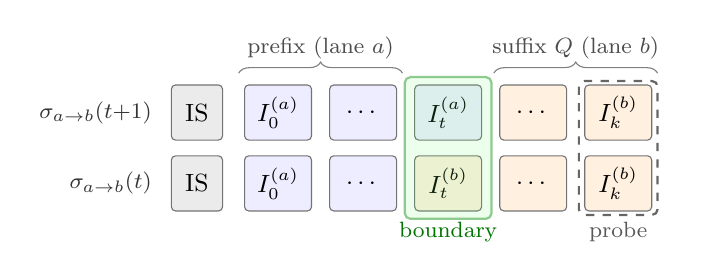
\begin{tikzpicture}[
  font=\small,
  cell/.style={draw=black!55, rounded corners=1.5pt, minimum width=8.5mm,
               minimum height=7mm, inner sep=1pt, align=center},
  acell/.style={cell, fill=blue!7},
  bcell/.style={cell, fill=orange!12},
  is/.style={cell, fill=black!8, minimum width=6.5mm},
  hdr/.style={font=\footnotesize, text=black!70},
  rl/.style={font=\footnotesize, text=black!80, anchor=east},
]
  \def\dx{1.08}
  \def\ya{0} \def\yb{-0.9}
  \path (-1.6,0) -- ({0.5+5*\dx+0.85},0);
  \node[rl] at (0.1,\ya) {$\spl{t{+}1}$};
  \node[is] at (0.55,\ya) {$\IS$};
  \node[acell] at ({0.5+1*\dx},\ya) {$\inp{0}{a}$};
  \node[acell] at ({0.5+2*\dx},\ya) {$\cdots$};
  \node[acell] at ({0.5+3*\dx},\ya) {$\inp{t}{a}$};
  \node[bcell] at ({0.5+4*\dx},\ya) {$\cdots$};
  \node[bcell] at ({0.5+5*\dx},\ya) {$\inp{k}{b}$};
  \node[rl] at (0.1,\yb) {$\spl{t}$};
  \node[is] at (0.55,\yb) {$\IS$};
  \node[acell] at ({0.5+1*\dx},\yb) {$\inp{0}{a}$};
  \node[acell] at ({0.5+2*\dx},\yb) {$\cdots$};
  \node[bcell] at ({0.5+3*\dx},\yb) {$\inp{t}{b}$};
  \node[bcell] at ({0.5+4*\dx},\yb) {$\cdots$};
  \node[bcell] at ({0.5+5*\dx},\yb) {$\inp{k}{b}$};
  \fill[green!60, fill opacity=0.12, rounded corners=2pt]
      ({0.5+3*\dx-0.55},{\ya+0.45}) rectangle ({0.5+3*\dx+0.55},{\yb-0.45});
  \draw[green!50!black, opacity=0.42, thick, rounded corners=2pt]
      ({0.5+3*\dx-0.55},{\ya+0.45}) rectangle ({0.5+3*\dx+0.55},{\yb-0.45});
  \node[hdr, text=green!45!black] at ({0.5+3*\dx},{\yb-0.62}) {boundary};
  \draw[black!60, thick, dashed, rounded corners=2pt]
      ({0.5+5*\dx-0.5},{\ya+0.4}) rectangle ({0.5+5*\dx+0.5},{\yb-0.4});
  \node[hdr, text=black!65] at ({0.5+5*\dx},{\yb-0.62}) {probe};
  \draw[decorate,decoration={brace,amplitude=4pt},black!50]
      ({0.5+1*\dx-0.5},{\ya+0.5}) -- ({0.5+2*\dx+0.5},{\ya+0.5});
  \node[hdr] at ({0.5+1.5*\dx},{\ya+0.82}) {prefix (lane $a$)};
  \draw[decorate,decoration={brace,amplitude=4pt},black!50]
      ({0.5+4*\dx-0.5},{\ya+0.5}) -- ({0.5+5*\dx+0.5},{\ya+0.5});
  \node[hdr] at ({0.5+4.5*\dx},{\ya+0.82}) {suffix $Q$ (lane $b$)};
\end{tikzpicture}
\caption{The two splices at a boundary $t$. They share $\IS$, the common prefix (lane $a$)
and the common suffix $Q$ (lane $b$), and differ only at column $t$.}
\label{fig:boundary}
\end{figure}

Reporting a genuine violation therefore reduces to finding a boundary, which we address next.

%===============================================================================
\subsection{Localizing the boundary}
\label{sec:detect-localize}
%===============================================================================

A flagged candidate shows only that the probe readings of the two lanes differ. It does not tell
which input pair causes it, and that pair may sit in any column up to the probe.
Localization finds it as a boundary, whose input pair is a genuine violation
(\S\ref{sec:detect-soundness}). Both localizers share one primitive, $\textsc{Measure}(t)$:
run $\batch{\spl{t}}$, repeated to reduce noise, and return $r(t)$. We run each localizer both as
$a\to b$ and as $b\to a$, and both are sound, so neither adds a false positive.

\begin{figure*}[t]
\begin{minipage}[t]{0.48\textwidth}
\begin{algorithm}[H]
\caption{Linear scan ($a\!\to\!b$), returns $\tmax$}
\label{alg:scan}
\begin{algorithmic}[1]
\State $\mathit{prev} \gets r(k{+}1)$ \Comment{lane $a$, known}
\For{$t \gets k$ \textbf{down to} $1$}
  \State $\mathit{cur} \gets \textsc{Measure}(t)$
  \If{$\mathit{cur} \neq \mathit{prev}$}
     \State \Return $t,\ (\inp{t}{a}, \inp{t}{b})$ \Comment{boundary}
  \EndIf
  \State $\mathit{prev} \gets \mathit{cur}$
\EndFor
\State \Return $0,\ (\inp{0}{a}, \inp{0}{b})$
\Statex
\end{algorithmic}
\end{algorithm}
\end{minipage}\hfill
\begin{minipage}[t]{0.48\textwidth}
\begin{algorithm}[H]
\caption{Binary search ($a\!\to\!b$)}
\label{alg:binsearch}
\begin{algorithmic}[1]
\State $\ell \gets 0;\quad h \gets k{+}1$ \Comment{$r(\ell)\neq r(h)$, known}
\While{$h > \ell + 1$}
  \State $m \gets \lfloor (\ell+h)/2 \rfloor$
  \If{$\textsc{Measure}(m) \neq r(\ell)$}
     \State $h \gets m$ \Comment{boundary below $m$}
  \Else
     \State $\ell \gets m$ \Comment{boundary above $m$}
  \EndIf
\EndWhile
\State \Return $\ell,\ (\inp{\ell}{a}, \inp{\ell}{b})$
\end{algorithmic}
\end{algorithm}
\end{minipage}
\end{figure*}

A \emph{linear scan} (Algorithm~\ref{alg:scan}) walks the splits down from the probe end and stops
at the first neighboring pair that disagrees. It runs at most $k$ measurements and returns the
highest boundary $\tmax$. Without the early stop, it continues and reports every leaking column. A
\emph{binary search} (Algorithm~\ref{alg:binsearch}) returns a single boundary in
$\lceil\log_2(k+1)\rceil$ measurements, by keeping a window whose end readings differ and halving
it at each step. Both localizers have matching lower bounds, so each is optimal for what it
returns. The linear scan is optimal among localizers that must return $\tmax$, and the binary
search among those that must return some boundary. Appendix~\ref{app:localize} gives a worked
example and the lower-bound proofs.

Our implementation defaults to a galloping variant, which probes at doubling distances from the
probe end before running a binary search over the bracketed range. It helps when a boundary lies
near the probe, which is common because the most recent inputs often cause the leak, and otherwise
costs a small constant factor more than the plain binary search.

%===============================================================================
\subsection{Generalizing priming}
\label{sec:detect-priming}
%===============================================================================

Without lanes, \textsc{Revizor} keeps boosted and original inputs in one flat sequence,
and priming validates a flagged pair by swapping its two positions. With lanes, the two
inputs of a flagged pair occupy the same column of two lanes. Priming's two comparisons
(Eq.~\eqref{eq:priming}) then coincide with the first step of the linear scan in each direction.
The first compares $\spl{k{+}1}=\lane{a}$ with $\spl{k}$, which swaps in only $\inp{k}{b}$, and
the second compares $\sigma_{b\to a}(k{+}1)=\lane{b}$ with $\sigma_{b\to a}(k)$. Priming stops
there and discards the candidate if both pairs agree, whereas the scan continues and reports the
boundaries priming misses. On the Neoverse~N3, the scan finds the BTB-carried canonicality leak
in $84$\,s on average, while priming misses it throughout a 48-hour campaign
(Table~\ref{tab:violations}).

A drawback is that lanes compare inputs only within a column, whereas the flat sequence lets
priming compare any two positions. Our generalization therefore misses violations between two
inputs of the same lane. Such pairs are rare. According to the measurements of~\cite{hide_seek},
fewer than $6\%$ of random inputs share a contract trace on x86, and none do for test cases with
at least $16$ memory accesses. This rarity was the original motivation for boosting.
\todo{Is ``generalization'' the right term? Lanes do not keep priming's within-lane comparisons.}

%-------------------------------------------------------------------------------
\section{Porting \textsc{Revizor} to AArch64}
\label{sec:port}
% Preamble: \usepackage{tikz}  \usetikzlibrary{arrows.meta,calc}
%           \newif\ifshowspectree \showspectreetrue
%           \newif\ifshowexecfsm  \showexecfsmtrue
%-------------------------------------------------------------------------------
\textsc{Revizor}~\cite{revizor} is a pipeline of four components, a generator, a model, an
executor, and an analyzer, of which only the first three depend on the ISA. We keep the
pipeline, rebuild these three for AArch64, and add support for Pointer Authentication and MTE.
We evaluate the port in \S\ref{sec:eval}.

\paragraph{Components.}
Mainline \textsc{Revizor} models the contract by default by emulating the test case in software.
We execute the test case natively on an AArch64 host core, inside a separate process, the
\emph{contract executor} (CE). The hardware trace comes from a Linux kernel module, which runs
the test case on the CPU under test and measures its footprint (Figure~\ref{fig:components}).

\paragraph{Instruction set from the architecture specification.}
Mainline \textsc{Revizor} reads its instruction table from a prebuilt file. We build ours
automatically from Arm's machine-readable A64 specification, which describes each instruction's
encoding, operands, and behavior. Instructions whose description we cannot fully recover are
excluded, so the generator uses only instructions it models
completely. Pinning the specification release keeps this set reproducible.

\paragraph{Remote fuzzing.}
Arm cores commonly ship inside phones and embedded devices that cannot host the generation,
modeling, and analysis stack. We keep those on a capable host and leave the device only the
execution and measurement that need its silicon, reached over SSH or ADB. Running the heavy
generation and modeling on the host rather than the device speeds up fuzzing.

\paragraph{Contract executor: native single-stepping.}
\label{component:CE}
Rather than emulating AArch64, the CE executes the test case natively on an AArch64 host core
and single-steps it (Figure~\ref{fig:trampoline}). It loads the program into an executable
mapping and relies on the fixed-width A64 encoding: every instruction is 32 bits, and so is a
\texttt{BL} branch. The CE can therefore overwrite any instruction word in place with a
\texttt{BL} to a trampoline. To run one instruction, it restores that instruction at the current
program counter, while every other word still holds a trampoline branch. The core executes the
instruction natively and then takes the next \texttt{BL} into the trampoline, which saves the
registers and condition flags and records the architectural state. Because every \texttt{BL}
overwrites the link register, the CE keeps the test case's link register and call stack in
software. Running natively avoids the emulation inconsistencies we found in emulators such as
Unicorn~\cite{unicorn}. For the extensions, the CE uses a middle ground. It can model Pointer
Authentication and MTE in software, so a feature the host lacks is still covered without a full
emulator's fidelity gaps. For instance, we fuzzed MTE on a Google Pixel~8, which implements it,
while generating and modeling on a host that does not support MTE.

\begin{figure}[t]
\centering
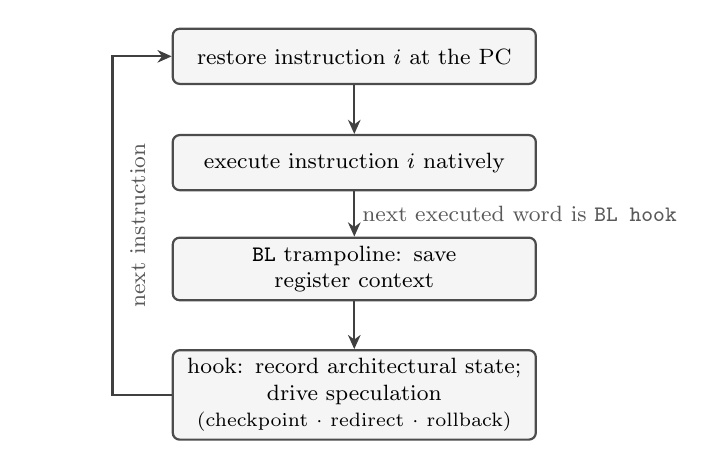
\begin{tikzpicture}[
  font=\footnotesize,
  stp/.style={draw=black!70, fill=black!4, rounded corners=2.5pt, thick,
              align=center, text width=44mm, minimum height=7mm, inner sep=3pt},
  ar/.style={-{Stealth[length=1.8mm,width=1.6mm]}, thick, draw=black!75},
  lbl/.style={font=\scriptsize, text=black!65, inner sep=1.5pt},
]
  \node[stp] (rs) at (0,0)    {restore instruction $i$ at the PC};
  \node[stp] (ex) at (0,-1.35){execute instruction $i$ natively};
  \node[stp] (tr) at (0,-2.7) {\texttt{BL} trampoline: save register context};
  \node[stp] (hk) at (0,-4.3){hook: record architectural state;\\ drive speculation\\ {\scriptsize (checkpoint $\cdot$ redirect $\cdot$ rollback)}};
  \draw[ar] (rs) -- (ex);
  \draw[ar] (ex) -- (tr) node[lbl,font=\footnotesize,midway,right=1pt]{next executed word is \texttt{BL hook}};
  \draw[ar] (tr) -- (hk);
  \draw[ar] (hk.west) -- ++(-0.75,0) |- (rs.west);
  \node[lbl, font=\footnotesize, rotate=90, fill=white, inner sep=1pt] at (-2.75,-2.15) {next instruction};
  % center on the box column, ignoring the return loop's leftward reach
  \path let \p1 = (current bounding box.north east),
            \p2 = (current bounding box.south west),
            \n1 = {max(\x1, -\x2)} in
        coordinate (bbne) at (\n1, \y1) coordinate (bbsw) at (-\n1, \y2);
  \pgfresetboundingbox
  \useasboundingbox (bbsw) rectangle (bbne);
\end{tikzpicture}
\caption{The CE single-steps the test case. After each native instruction, a
\texttt{BL} enters the trampoline, which records architectural state and drives
speculation emulation.}
\label{fig:trampoline}
\end{figure}
\paragraph{Execution clause and speculation stack.}
A contract's execution clause specifies what speculation the CE must model, and the CE realizes
it with a \emph{speculation stack}. At a speculation point, such as a mispredicted branch or a
bypassed store, the CE pushes a checkpoint, a snapshot of the registers, the sandbox memory, the
MTE tag memory, and the call stack, and redirects execution onto the speculative path. When that
path ends or exhausts its per-window instruction budget, the CE pops the checkpoint, restores the
snapshot, and resumes at the recorded address. Windows nest up to a configured depth, and an
inner window unwinds before the one enclosing it.

\ifshowspectree
\begin{figure}[t]
\centering
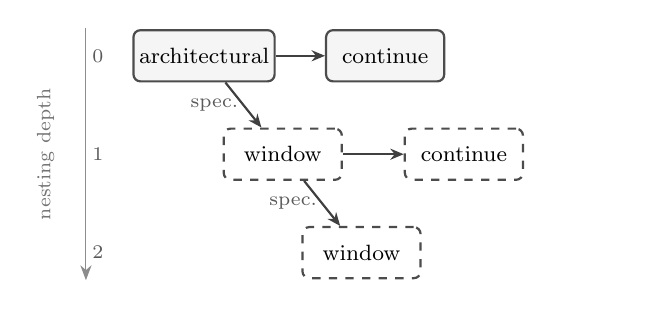
\begin{tikzpicture}[
  font=\footnotesize,
  w/.style={draw=black!70, fill=black!4, rounded corners=2.5pt, thick,
            align=center, minimum width=15mm, minimum height=6.5mm, inner sep=2pt},
  spec/.style={w, dashed, fill=white},
  e/.style={-{Stealth[length=1.7mm,width=1.4mm]}, thick, draw=black!75},
  lbl/.style={font=\scriptsize, text=black!65, inner sep=1.5pt},
  axis/.style={-{Stealth[length=1.9mm]}, draw=black!45},
]
  \draw[axis] (-1.5,0.35) -- (-1.5,-2.85);
  \node[font=\scriptsize, text=black!55, rotate=90, anchor=south] at (-1.78,-1.25) {nesting depth};
  \node[lbl, anchor=east] at (-1.22, 0)     {0};
  \node[lbl, anchor=east] at (-1.22,-1.25)  {1};
  \node[lbl, anchor=east] at (-1.22,-2.5)   {2};

  \node[w]    (w0) at (0,0)        {architectural};
  \node[w]    (a0) at (2.3,0)      {continue};
  \node[spec] (w1) at (1.0,-1.25)  {window};
  \node[spec] (a1) at (3.3,-1.25)  {continue};
  \node[spec] (w2) at (2.0,-2.5)   {window};

  \draw[e] (w0) -- (a0);
  \draw[e] (w0) -- (w1) node[lbl,midway,left=0pt]{spec.};
  \draw[e] (w1) -- (a1);
  \draw[e] (w1) -- (w2) node[lbl,midway,left=0pt]{spec.};

  % center on the box cluster (center x = 1.65cm), not the depth axis
  \path let \p1 = (current bounding box.north east),
            \p2 = (current bounding box.south west),
            \n1 = {max(\x1-1.65cm, 1.65cm-\x2)} in
        coordinate (bbne) at ({1.65cm+\n1}, \y1)
        coordinate (bbsw) at ({1.65cm-\n1}, \y2);
  \pgfresetboundingbox
  \useasboundingbox (bbsw) rectangle (bbne);
\end{tikzpicture}
\caption{Execution forks at each speculation point into a speculative window
(dashed) and the continuation. Windows nest to deeper levels and unwind innermost
first.}
\label{fig:spec-stack}
\end{figure}
\fi

\ifshowexecfsm
\begin{figure*}[t]
\centering
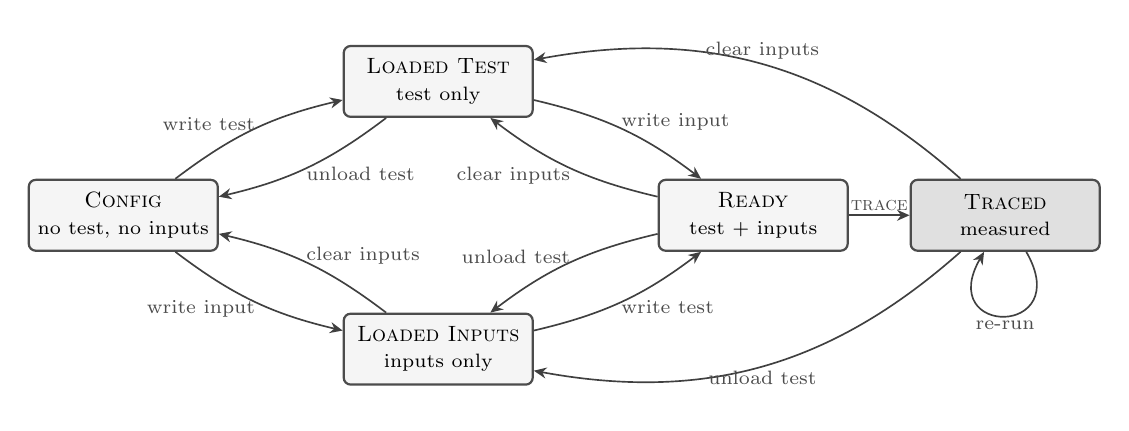
\begin{tikzpicture}[
  font=\footnotesize,
  st/.style={draw=black!70, fill=black!4, rounded corners=2.5pt, thick,
             align=center, minimum width=24mm, minimum height=9mm, inner sep=2pt},
  fin/.style={st, fill=black!12},
  ed/.style={-{Stealth[length=1.6mm,width=1.4mm]}, semithick, draw=black!75},
  lbl/.style={font=\scriptsize, text=black!70, inner sep=1.5pt},
]
  \node[st]  (cfg) at (0,0)      {\textsc{Config}\\{\scriptsize no test, no inputs}};
  \node[st]  (lt)  at (4.0,1.7)  {\textsc{Loaded Test}\\{\scriptsize test only}};
  \node[st]  (li)  at (4.0,-1.7) {\textsc{Loaded Inputs}\\{\scriptsize inputs only}};
  \node[st]  (rdy) at (8.0,0)    {\textsc{Ready}\\{\scriptsize test + inputs}};
  \node[fin] (tr)  at (11.2,0)   {\textsc{Traced}\\{\scriptsize measured}};

  \draw[ed] (cfg) to[bend left=12]  node[lbl,above left=-3pt]{write test}   (lt);
  \draw[ed] (lt)  to[bend left=12]  node[lbl,below right=-3pt]{unload test} (cfg);
  \draw[ed] (cfg) to[bend right=12] node[lbl,below left=-3pt]{write input}  (li);
  \draw[ed] (li)  to[bend right=12] node[lbl,above right=-3pt]{clear inputs} (cfg);
  \draw[ed] (lt)  to[bend left=12]  node[lbl,above right=-3pt]{write input} (rdy);
  \draw[ed] (rdy) to[bend left=12]  node[lbl,below left=-3pt]{clear inputs} (lt);
  \draw[ed] (li)  to[bend right=12] node[lbl,below right=-3pt]{write test}  (rdy);
  \draw[ed] (rdy) to[bend right=12] node[lbl,above left=-3pt]{unload test}  (li);
  \draw[ed] (rdy) -- node[lbl,above]{\textsc{trace}} (tr);
  \draw[ed] (tr) to[out=-60,in=-120,looseness=6] node[lbl,below]{re-run} (tr);
  \draw[ed] (tr) to[bend right=26] node[lbl,above]{clear inputs} (lt);
  \draw[ed] (tr) to[bend left=26]  node[lbl,below]{unload test}  (li);
\end{tikzpicture}
\caption{Executor state machine. A run is possible only in \textsc{Ready}.}
\label{fig:executor-fsm}
\end{figure*}
\fi

\paragraph{Driving the executor.}
The fuzzer drives the kernel module through a character device. A test case and its inputs are
written to the device independently, a run is possible once both are loaded, and re-running a
loaded test case re-measures all its inputs. Per input, a run returns a bitmap of the L1D cache
sets it touched. \texttt{sysfs} attributes configure the rest, including the measurement method
(Prime+Probe or Flush+Reload), the pinned core, the number of warm-up runs, whether speculative
store bypass is enabled, and other executor settings.

\paragraph{REIF (Revizor Extensible Input File).}
Each input is stored as a self-describing \texttt{.reif} file made of typed sections, so new
per-input state can be added without changing the format. The required sections hold the
initial register values and the sandbox memory. Optional sections carry further state, such as
custom PAC keys, the initial MTE tag memory, and the global value table introduced in
\S\ref{sec:precond}. The kernel module and the CE consume the same file, so the model and the
hardware start from an identical initial state.

%-------------------------------------------------------------------------------
\section{Evaluation}
\label{sec:eval}
%-------------------------------------------------------------------------------

\paragraph{Setup.}
Our primary target is an Arm Neoverse~N3 (Armv9.2-A). We reproduce the Arm-specific leaks
on a Google Pixel~8 (Tensor~G3), pinning to its Cortex-A715 (Armv9.0-A) and Cortex-X3 cores in
turn, and run the MTE experiments on the Pixel~8 only. We use an Intel
Alder Lake core as a non-Arm baseline. Following prior Revizor
work~\cite{revizor,revizor_micro,hide_seek}, we report throughput as test cases
per hour with the number of inputs per test case, and we report, per discovered
violation, the \emph{time to detection} (TTD): the mean wall-clock time before the
first detected violation, over $20$ independent fuzzing runs.

\subsection{Fuzzing throughput}
\label{sec:eval-throughput}
Our fuzzer runs in two configurations. In \emph{local} execution the generator, contract
executor, and hardware executor all run on the N3. In \emph{remote} execution the N3 generates
and models test cases while a thin agent on each device only executes them and returns
\texttt{HTrace}s. This lets one controller drive devices that cannot host the full toolchain,
such as the Pixel~8's Cortex-A715. The N3 reaches that device over an SSH tunnel and the
Android Debug Bridge (ADB).
Table~\ref{tab:throughput} reports both.
For context, Revizor on x86 sustains over $200$ test cases per hour for complex
contracts, with several hundred inputs per test case~\cite{revizor,revizor_micro}.
\todo{measure and update: the x86 \textsc{Revizor} $200$ tc/hour figure is likely outdated.}

\begin{table}[t]\centering\small
\setlength{\tabcolsep}{6pt}
\caption{Fuzzing throughput: local execution on the Neoverse~N3 versus remote execution on the
Pixel~8's Cortex-A715 driven from the N3. \emph{tc/s} is test cases generated and measured per
second, \emph{traces/s} is hardware input measurements per second.}
\label{tab:throughput}
\begin{tabular}{@{}lcc@{}}
\toprule
 & Local & Remote \\
\midrule
tc/s               & $0.94$  & $0.17$ \\
traces/s           & $1962$  & $414$ \\
Inputs / test case & $100$   & $100$ \\
\bottomrule
\end{tabular}
\end{table}

\subsection{Contract violations}
\label{sec:eval-violations}
Table~\ref{tab:violations} lists the violations we find and whether each
reproduces on the N3, the Pixel~8, and the Alder Lake baseline. Spectre-v1 (conditional branch) and Spectre-v4 (speculative store bypass) are not a
contribution of this work. We reproduce them as a sanity check~\cite{revizor}. For Spectre-v2
(indirect branch), the leak is detected Revizor-style through the L1D, because the
target function uses an unused register. Our own leak findings are two Arm-specific leaks, the
\emph{canonicality} leak and the \emph{AUT*} sign-bit leak. Speculative-exception fuzzing also
rediscovers TikTag~\cite{tiktag} on the Pixel~8, and on the Alder Lake baseline the
source-agnostic detection surfaces the known AfterImage IP-prefetcher leak~\cite{afterimage}.

\paragraph{Canonicality.}
\label{sec:canon-l1d}
On AArch64, address translation accepts a virtual address only when the bits above the
configured virtual-address size are all zero (the TTBR0 range) or all one (the TTBR1 range).
Any other value is out of range and faults~\cite{arm_vmsa}. On the
Neoverse~N3 and the Cortex-A715, a speculative access to a canonical target allocates
\uarch state as usual (an L1D line, a data or instruction TLB entry, a BTB
way), whereas an \emph{out-of-range} target is fast-rejected before it allocates
anything and leaves no footprint. The presence or absence of that footprint is thus a one-bit
oracle on the canonicality of the accessed pointer. The same fast-reject covers
alignment. A speculative access that is misaligned for its access type is rejected
before it allocates. An SP-relative access requires 16-byte alignment and a
PC-relative or indirect-branch target requires 4-byte alignment, so the oracle equally
reports whether a computed address carries the correct low alignment bits.
The canonicality leak surfaces on the N3. Its cache and TLB channels are not exclusive to Arm.
They rest on a rule that is not Arm-specific, namely that a non-canonical access is rejected
before it allocates any \uarch state, and they reproduce on the Intel Alder
Lake. Its BTB channel applies the same rule to a branch target, that a non-canonical
target is rejected before it allocates a BTB entry. It is narrower, as it reproduces on the N3
and the Pixel~8's Cortex-A715 but not on Alder Lake or the Cortex-X3, where speculative BTB
allocation shows no in-range versus out-of-range distinction, indicating this behaviour is
\uarch-dependent (Table~\ref{tab:violations}).

\paragraph{AUT* sign bit.}
The \texttt{AUT*} instruction family leaks the pointer's \emph{sign bit}, not its signature.
To mitigate PACMAN-style attacks~\cite{pacman}\,\cite{arm_pacman}, Arm makes speculative
authentication proceed as if the PAC were correct regardless of its value. The architecture then sign-extends the effective
sign bit into the bits the \texttt{PAC} field occupied, just before the access, so a corrupted
sign bit leaves no footprint in the L1D, data TLB, or instruction TLB, unlike a correct one. This
holds for both \texttt{AUT*} and the combined authenticate-and-branch instructions, so any value
passed to an authentication instruction leaks its bit~55, a one-bit-per-call primitive. The
\texttt{RETA*} and \texttt{BLRA*} instructions that carry it appear throughout the Linux kernel.

\paragraph{An IP-prefetcher leak on Alder Lake.}
On the Intel Alder Lake baseline we also surface a leak no contract models, carried by the L1
data-cache IP-stride prefetcher. A load whose target address depends on a secret trains the
prefetcher, which runs ahead and pulls a secret-dependent line into the cache, outside the
contract's account of the program's own accesses. The channel is gated entirely by that
prefetcher: it appears and disappears deterministically as the IP-prefetcher control bit
(MSR~\texttt{0x1A4} bit~3) is toggled, and is the known AfterImage channel~\cite{afterimage}.
Surfacing a genuine leak on a non-Arm core shows the method is not Arm-specific.

\paragraph{TikTag on the Pixel~8.}
To fuzz the speculative MTE tag-check condition, we use the window-widening template of
\S\ref{sec:precond} (Figure~\ref{fig:tiktag-tmpl}). It rediscovers TikTag-v1, an MTE tag leak
through speculation shrinkage~\cite{tiktag}, which we detect on the Cortex-X3 but not the
Cortex-A715, matching Kim et al.~\cite{tiktag}.

\begin{table*}[t]\centering\small
\setlength{\tabcolsep}{4pt}
\caption{Contract violations, the configuration that finds each (method and whether the
source-agnostic rule is what flags it), their time to first detection (TTD), and where each
reproduces. \cmark/\xmark\ in the platform columns: reproduced / not observed. \emph{n/a}: the
feature is not available on that platform.}
\label{tab:violations}
\begin{tabular}{@{\hspace{6pt}}l l c l c c c c c@{\hspace{6pt}}}
\toprule
Violation & Method & Src-agn. & Channel & TTD & N3 & A715 & X3 & Alder Lake \\
\midrule
Spectre-v1 (conditional branch) & baseline & \xmark & L1D cache & $53.9$\,s$^{\dagger}$   & \cmark & \cmark & \cmark & \cmark \\
Spectre-v2 (indirect branch)    & baseline & \xmark & L1D cache & $25$\,min$^{\dagger}$   & \cmark & \cmark & \cmark & \cmark \\
Spectre-v4 (store bypass)       & baseline & \xmark & L1D cache & $32.3$\,s$^{\dagger}$   & \cmark & \cmark & \cmark & \cmark \\
Canonicality                    & spec-exc & \xmark & L1D cache & $42.9$\,s$^{\dagger}$   & \cmark & \cmark & \cmark & \cmark \\
Canonicality                    & spec-exc & \cmark & BTB       & $84.0$\,s$^{\dagger}$   & \cmark & \cmark & \xmark & \xmark \\
\texttt{AUT*} sign bit          & spec-exc & \xmark & L1D cache & $54.5$\,s$^{\dagger}$   & \cmark & \cmark & \cmark & n/a \\
TikTag-v1 (MTE tag check)~\cite{tiktag} & spec-exc\,+\,tmpl & \xmark & L1D cache & $131.9$\,s$^{\ddagger}$ & n/a$^{\S}$ & \xmark & \cmark & n/a \\
L1D IP prefetcher~\cite{afterimage} & baseline & \cmark & HW-pref.  & $35$\,min$^{\P}$     & \xmark & \xmark & \xmark & \cmark \\
\bottomrule
\end{tabular}

\smallskip
\footnotesize
\emph{Method}: \emph{baseline} is standard relational fuzzing, \emph{spec-exc} is
speculative-exception fuzzing (\S\ref{sec:precond}), and $+\,$tmpl adds the window-widening
template (Figure~\ref{fig:tiktag-tmpl}). \emph{Src-agn.}\ (\cmark): the leak is flagged by the
source-agnostic detection rule rather than on a modeled channel.\\
$^{\dagger}$Mean over $20$ seeds on the Neoverse~N3.
$^{\ddagger}$Mean over $20$ seeds on the Cortex-X3.
$^{\S}$The N3 reports FEAT\_MTE but not FEAT\_MTE2, so it keeps no Allocation Tags in
memory and performs no tag checks, leaving nothing for TikTag to leak.
$^{\P}$A single campaign on Alder Lake.
\end{table*}

\subsection{Reach across isolation boundaries}
\label{sec:eval-reach}
Table~\ref{tab:reach} reports, for each boundary and transmitting structure, the rate at which an unprivileged
attacker recovers one bit over the \texttt{cntvct\_el0} counter. The transmitting structures are complementary:
the iTLB crosses a thread and the EL2-to-EL0 boundary, the BTB crosses a process and a VM, and the
blanks are structural, at chance even under the PMU. A BTB set is set-associative, so
reliably marking it takes several branches~\cite{indirector}, and the victim issues $64$ branches to
the same set. The canonicality leak transmits the bit through bit~48 of the pointer, and the
\texttt{AUT*} leak through bit~55. Every transmitting structure except the dTLB leaks any bit above the
virtual-address size, while the dTLB leaks only bit~48. When Top Byte Ignore (TBI)~\cite{arm_tbi} is
enabled, the fast-reject check ignores the top byte, so a bit placed there cannot be leaked. The
dagger cells reach $100\%$ only under the privileged PMU, which counts the event rather than timing
it with the coarse \texttt{cntvct\_el0} counter.

\begin{table}[t]\centering\footnotesize
\setlength{\tabcolsep}{5pt}
\caption{Reach of each transmitting structure across isolation boundaries on the Neoverse~N3. Each cell is the
unprivileged \texttt{cntvct\_el0} rate with per-bit error over $20$ runs. \xmark\ marks no
channel, at chance even under the PMU. A dagger marks a cell noisy on \texttt{cntvct\_el0} but reliable under the privileged PMU (dTLB
$3{,}922$, BTB $4{,}722$ bit/s). Rates are for the canonicality leak. The \texttt{AUT*} leak
coincides except on the BTB, which it does not reach.}
\label{tab:reach}
\begin{tabular}{@{}l r r r@{}}
\toprule
 & \multicolumn{3}{c}{[bits/s] (error \%)} \\
\cmidrule(lr){2-4}
Victim $\to$ attacker & dTLB & iTLB & BTB \\
\midrule
Cross-thread (EL0)                & $144\ (24\%)^{\dagger}$ & $1{,}269\ (3\%)$ & $6\ (31\%)^{\dagger}$ \\
Cross-process (EL0$\to$EL0)       & \xmark                  & \xmark           & $18\ (0\%)$ \\
Cross-EL (EL2$\to$EL0)            & $97\ (31\%)^{\dagger}$  & $1{,}400\ (1\%)$ & \xmark \\
Cross-VM (host $\to$ VM)          & \xmark                  & \xmark           & $11\ (0\%)$ \\
\bottomrule
\end{tabular}
\end{table}

\subsection{Localization cost}
\label{sec:eval-localize}
Once a violation is detected, we localize the responsible boundary among the
$k$ columns of a priming batch (\S\ref{sec:detect-localize}).
We measure each localizer by placing the single leaking boundary at each of the $k+1$
possible positions in turn and averaging the interior splices it issues, the two bracket
readings being already known from the flagged candidate. For $k=12$, $64$, and $256$, the
linear scan runs at most $k$ probes and averages $6.92$, $33.0$, and $129.0$, while the
binary search runs $\lceil\log_2(k{+}1)\rceil$ probes ($4$, $7$, and $9$) and averages
$3.77$, $6.03$, and $8.01$, at or just below that bound.

%-------------------------------------------------------------------------------
\section{Demonstrating the canonicality leak}
\label{sec:canon}
%-------------------------------------------------------------------------------
We build two independent demonstrations of the canonicality leak used as a covert channel. The
OpenSSL demonstration is dynamically
linked and built with Pointer Authentication and stack canaries disabled, with a single vulnerable
\texttt{memcpy} planted in it. The canary demonstration keeps both enabled.

\textbf{OpenSSL RSA key.} A plain stack-buffer overflow drives a ROP chain built
\emph{entirely from gadgets inside the OpenSSL library itself}, opening a Spectre-v4
window and transmitting over the BTB channel, which we read with the low-privilege
\texttt{cntvct\_el0} counter~\cite{riscyrop}. Because the read primitive walks OpenSSL's
own heap, it recovers a complete, in-use RSA-2048 private key at \texttt{--samples 1500},
in about $3$~h.

\textbf{Blind stack-canary recovery.} A single two-dimensional-array gadget, driven by
three distinct speculation primitives, recovers a victim's stack canary with no prior
knowledge of its value. The oracle recovers bits \texttt{[55:0]} of the 64-bit canary.
The top byte \texttt{[63:56]} is ignored under TBI~\cite{arm_tbi} and cannot be leaked. The proof of concept assumes every
page the probe reaches is mapped. The victim explicitly maps, at startup, the finite set
of pages the probe needs, since mapping the entire user address space is not practical.
Address translation mechanisms such as paging determine whether a page is mapped. That is an
allocation outcome, and the canary's secrecy should not rest on it.

%-------------------------------------------------------------------------------
\section{Related Work}
\label{sec:related}
%-------------------------------------------------------------------------------

\paragraph{Model-based relational testing.}
\textsc{Revizor} established black-box relational testing against speculation contracts,
finding Spectre-V1, Spectre-V4, MDS, and LVI-Null leaks on
x86-64~\cite{revizor,revizor_micro}, and later work scaled the search and modeled
exception-driven, isolation-boundary, and pre-silicon
leakage~\cite{hide_seek,speculation_fault,isolation,amulet}. All keep every faulting
instruction safe for all inputs, so a condition is never violated, even transiently. We
instead satisfy a condition on the committed path and violate it only on a transient path, and detect leaks whose transmitting structure is never the observed L1D. On Arm,
Scam-V validated abstract side-channel models on an in-order
Cortex-A53~\cite{scamv,scamv_micro}. Ours is the first relational tester on
out-of-order Arm server and mobile cores, and the first to fuzz operand conditions.

\paragraph{Arm speculative attacks.}
PACMAN~\cite{pacman} and TikTag~\cite{tiktag} attack Arm's Pointer Authentication
and Memory Tagging with hand-crafted gadgets, whereas our \texttt{AUT*} and
canonicality leaks fall out of the fuzzer automatically, which also rediscovers
TikTag-v1. The \texttt{AUT*} leak is orthogonal to Arm's FEAT\_FPACC\_SPEC
mitigation~\cite{arm_fpacc_spec}, leaking bit~55 key-independently. AMD's transient non-canonical
loads (CVE-2020-12965)~\cite{noncanonical_amd,amd_sb1010} stay within one domain, while ours
cross isolation boundaries.

\paragraph{Prefetcher and predictor channels.}
AfterImage leaks control flow through Intel's IP-stride L1D
prefetcher~\cite{afterimage}, and Augury and GoFetch exploit Apple's
data-memory-dependent prefetcher~\cite{augury,gofetch}. The Alder Lake channel our
method surfaces is AfterImage-style. BranchScope reads conditional-branch direction
from the pattern history table~\cite{branchscope}, and Branch History Injection reuses
branch history across privilege to defeat eIBRS and Arm CSV2~\cite{bhi}. Our source-agnostic
method treats such predictor-resident state as a transmitting structure that reaches L1D.

\paragraph{Pre-silicon fuzzing.}
IntroSpectre~\cite{introspectre}, SpecDoctor~\cite{specdoctor},
TEESec~\cite{teesec}, Phantom Trails~\cite{phantom_trails}, and
DejaVuzz~\cite{dejavuzz} find transient-execution bugs in open RISC-V designs
with full RTL visibility. We instead test commercial Arm silicon as a black box,
where most \uarch state is unobservable, and chain our gadgets with a
symbolic search in the spirit of RiscyROP~\cite{riscyrop}.

%-------------------------------------------------------------------------------
\section{Conclusion}
\label{sec:conclusion}
%-------------------------------------------------------------------------------
We brought model-based relational testing to AArch64, with a contract executor on the target
core and support for Pointer Authentication and MTE.
Speculative-exception fuzzing reaches the transient condition violations behind PACMAN and
TikTag without faulting the test case, and a source-agnostic rule provably reports leaks
whose L1D effect surfaces only in a later run. These uncovered two new speculative
covert-channel leaks on production Arm cores, in the address-range and alignment checks and
in Pointer Authentication's sign extension, recovered across isolation boundaries.

%-------------------------------------------------------------------------------
\section*{Acknowledgments}
%-------------------------------------------------------------------------------
We thank the anonymous reviewers for their valuable feedback. This research was conducted in collaboration with [redacted for review].
 


{\footnotesize \bibliographystyle{plain}
\bibliography{refs}}

\appendix
% Depends on the same preamble macros (\Al \AQ \lane \inp \spl \IS \tmax).
%===============================================================================
\section{Fuzzer component map}
\label{app:components}
Figure~\ref{fig:components} shows the component layout summarized in \S\ref{sec:port}.

\begin{figure}[H]
\centering
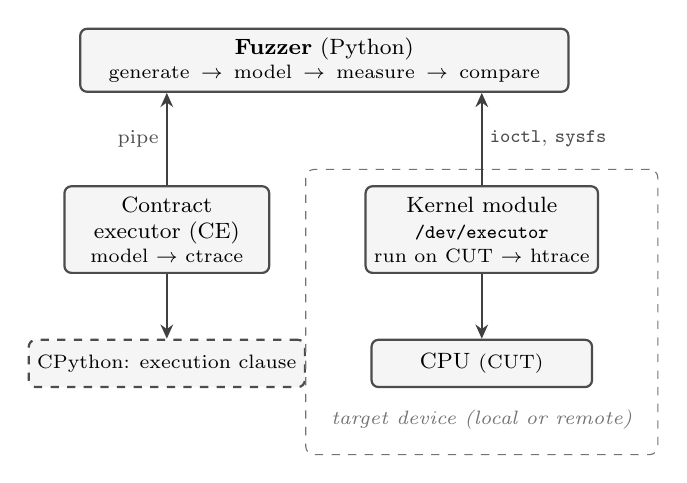
\begin{tikzpicture}[
  font=\footnotesize,
  box/.style={draw=black!70, fill=black!4, rounded corners=2.5pt, thick,
              align=center, inner sep=3pt},
  ch/.style={font=\scriptsize, text=black!70, align=center, inner sep=1.5pt},
  ar/.style={-{Stealth[length=1.8mm,width=1.6mm]}, thick, draw=black!75},
]
  \node[box, minimum width=62mm, minimum height=8mm] (fz) at (0,0)
    {\textbf{Fuzzer}~\textnormal{(Python)}\\[-1pt]%
     {\scriptsize generate \,$\to$\, model \,$\to$\, measure \,$\to$\, compare}};
  \node[box, minimum width=26mm, minimum height=11mm] (ce) at (-2.0,-2.15)
    {Contract\\executor (CE)\\[-1pt]{\scriptsize model $\to$ ctrace}};
  \node[box, minimum width=28mm, minimum height=11mm] (km) at (2.0,-2.15)
    {Kernel module\\{\scriptsize \texttt{/dev/executor}}\\[-1pt]{\scriptsize run on CUT $\to$ htrace}};
  \node[box, dashed, minimum width=26mm, minimum height=6mm] (bpu) at (-2.0,-3.85)
    {{\scriptsize CPython: execution clause}};
  \node[box, minimum width=28mm, minimum height=6mm] (cpu) at (2.0,-3.85)
    {CPU {\scriptsize (CUT)}};

  % target-device boundary (may be local or remote)
  \node[font=\scriptsize\itshape, text=black!55, below=1.5mm of cpu] (tdl)
    {target device (local or remote)};
  \node[draw=black!55, dashed, rounded corners=3pt, inner sep=2mm,
        fit=(km)(cpu)(tdl)] {};

  \draw[ar] (ce.north) -- (ce.north |- fz.south) node[ch,midway,left=1pt]{pipe};
  \draw[ar] (km.north) -- (km.north |- fz.south)
        node[ch,midway,right=1pt]{\texttt{ioctl}, \texttt{sysfs}};
  \draw[ar] (ce) -- (bpu);
  \draw[ar] (km) -- (cpu);
\end{tikzpicture}
\caption{Component map. The kernel module runs on the target device, local or
remote.}
\label{fig:components}
\end{figure}

%===============================================================================
\section{Proof-of-concept artifacts}
\label{app:pocs}
% TODO camera-ready: replace the withheld-link footnote with the public artifact repository URL.
We release the proof-of-concept programs behind our results at an anonymized
repository.\footnote{Link withheld for double-blind review.} Each is
\emph{self-scoring}: the victim draws a fresh random secret each round and the harness
compares it to the recovered value only for scoring. All measurements are on the
Neoverse~N3, pinned to isolated cores. The attacker runs unprivileged at EL0, and for
the cross-process and cross-VM cases it shares one physical core with the victim.
No elevated privilege, special instruction, or configuration is required beyond a
vulnerable code pattern and co-location on a core.

\paragraph{Cross-boundary PoC.} \texttt{cross\_boundary --switch \{aut|\allowbreak canon\}
--boundary \{same|\allowbreak xthread|\allowbreak xproc|\allowbreak xel|\allowbreak xvm\}} recovers a fresh random secret the attacker does not
know in advance, carried across an isolation boundary by the chosen channel. A
pointer-authentication signature supplies the secret, the 7-bit field \texttt{[54:48]} it writes
into a signed pointer, used here as a source of per-round randomness. Each round the victim signs
a pointer and, inside one Spectre-v4 store-bypass window, accesses it, and a bitmap the attacker
supplies routes one field bit to the position the chosen mechanism tests. The \texttt{canon} switch leaves that bit canonical or non-canonical, and
\texttt{aut} places it at bit~55 and authenticates, so the pointer stays in the user half or
sign-extends into the kernel half. The read-out runs over the L1D, data or instruction TLB, or
BTB (\texttt{--medium}), timed by a PMU event counter or the low-privilege \texttt{cntvct\_el0}
virtual counter (\texttt{--timer}).

\paragraph{Blind stack-canary recovery.} \texttt{canary\_leak\_blind -w \{v1|v4|rsb\}}
recovers a process's own stack canary with no prior knowledge of its value, from a
two-dimensional-array gadget driven by Spectre-v1, Spectre-v4, or Spectre-RSB, reading
the canonicality oracle through Flush+Reload~\cite{flushreload} over a pre-mapped array of
probe pages.

\paragraph{RSA-2048 key recovery through OpenSSL.} \texttt{rsa\_leak} recovers the bytes of
an in-use RSA-2048 private key from OpenSSL built with its ROP mitigations disabled and a
single planted vulnerable \texttt{memcpy}. A stack-buffer overflow drives a return-oriented chain built
entirely from OpenSSL's own gadgets, fires a Spectre-v4 window, and transmits over the BTB
channel read with \texttt{cntvct\_el0}.

\paragraph{An EL3 round trip does not flush the BTB.} \texttt{smc\_bench} tests a
condition for crossing the secure boundary. It primes one EL0 BTB entry, performs an
EL3 round trip between prime and probe, and reports that the entry survives, so an EL3
world switch does not by itself destroy the prediction state the BTB channel relies on.

%===============================================================================
\section{The window-widening template}
Figure~\ref{fig:tiktag-tmpl} gives the window-widening template of \S\ref{sec:precond} in full. The
\texttt{.macro.random\_instructions} entries are placeholders the fuzzer expands with fresh random
instructions for each test case.

\begin{figure}[H]
\centering
\begin{minipage}{0.92\linewidth}
\footnotesize
\begin{verbatim}
.function_0:
.bb_0.0:
  .macro.random_instructions.8.2.0:
  SDIV  x9, x1, x2        // 8-deep dependent
  SDIV  x9, x9, x2        //   chain: x9 resolves
  SDIV  x9, x9, x2        //   late, so the branch
  SDIV  x9, x9, x2        //   is predicted
  SDIV  x9, x9, x2
  SDIV  x9, x9, x2
  SDIV  x9, x9, x2
  SDIV  x9, x9, x2
  .macro.random_instructions.8.2.1:
  ORR   x9, x9, #1        // x9 odd => branch taken
  CBNZ  x9, .bb_0.2       //   (shadow is bb_0.1)
.bb_0.1:                  // mispredicted shadow:
  .macro.random_instructions.24.12.2:   // sealed
.bb_0.2:
  .macro.random_instructions.8.2.4:
\end{verbatim}
\end{minipage}
\caption{The window-widening template.}
\label{fig:tiktag-tmpl}
\end{figure}

%===============================================================================
\section{Localization analysis}
\label{app:localize}

Both localizers of \S\ref{sec:detect-localize} use the primitive $\textsc{Measure}(t)$,
which runs the batch $\batch{\spl{t}}$ and returns the probe reading $r(t)$. We show each localizer is optimal for what it returns
and summarize the trade-off in Table~\ref{tab:localizers}.

\subsection{Linear scan}
\label{app:scan}
The scan (Algorithm~\ref{alg:scan}) walks the split backwards from the probe end. From
the known $r(k+1)$ it measures $r(k),r(k-1),\dots$ and stops at the first neighbour that
disagrees. That split is a boundary, and its column is the highest leaking column.



\begin{proposition}[cost of the scan]
\label{prop:scancost}
The linear scan returns $\tmax=\max\{t:r(t)\neq r(t+1)\}$ and runs at most $k$ batches.
\end{proposition}
\begin{proof}
\todo{should this be removed? moved to appendix? only explained?}
It stops at the first $t$, counting down from $k$, with $r(t)\neq r(t+1)$. Since it did
not stop earlier, $r(t+1)=\dots=r(k+1)$, so no split above $t$ is a boundary and
$t=\tmax$. The interior splices it runs lie among $\spl{k},\dots,\spl{1}$, at most $k$.
\end{proof}

\subsection{Binary search}
\label{app:binsearch}
Binary search (Algorithm~\ref{alg:binsearch}) keeps a window $[\ell,h]$ whose end
readings differ, so a boundary lies inside, and halves it until it spans one split.
Figure~\ref{fig:binsearch} runs it on $12$ inputs with the leak at column~$4$.



\begin{proposition}[binary search returns a genuine violation]
\label{prop:bsearch}
Binary search makes at most $\lceil\log_2(k+1)\rceil$ runs and returns a boundary. By
the argument of \S\ref{sec:detect-soundness} its pair is a genuine violation.
\end{proposition}
\begin{proof}
\todo{should this be removed? moved to appendix? only explained?}
The invariant $r(\ell)\neq r(h)$ holds initially and is preserved: if $r(m)\neq r(\ell)$
then $[\ell,m]$ has unequal ends, otherwise $r(m)=r(\ell)\neq r(h)$ and $[m,h]$ does.
Each step halves $h-\ell$, so from $k+1$ it reaches $1$ in at most
$\lceil\log_2(k+1)\rceil$ runs, ending with $h=\ell+1$ and $r(\ell)\neq r(\ell+1)$.
\end{proof}

\begin{figure*}[p]
\centering
\newcommand{\bsrow}[4]{%
  \node[font=\scriptsize,anchor=east] at (-0.45,#1) {#3};
  \node[ci] at (0,#1) {IS};
  \foreach \c in {0,...,10}{
    \pgfmathsetmacro{\x}{0.68*(\c+1)}
    \ifnum\c<#2 \node[ca] at (\x,#1) {$\inp{\c}{a}$};
    \else       \node[cb] at (\x,#1) {$\inp{\c}{b}$}; \fi}
  \ifnum#2=12 \node[pa] at (8.16,#1) {$\inp{11}{a}$};
  \else       \node[pb] at (8.16,#1) {$\inp{11}{b}$}; \fi
  \node[font=\scriptsize,anchor=west] at (8.6,#1) {#4};}
\newcommand{\bsneq}[2]{%
  \draw[culprit,line width=1pt] (10.05,#1) -- (10.25,#1) -- (10.25,#2) -- (10.05,#2);
  \node[culprit,font=\small,anchor=west] at (10.25,{(#1+#2)/2}) {$\neq$};}
\newcommand{\bswin}[5]{%
  \draw[culprit,line width=1.1pt] ({0.68*(#3+1)-0.37},#1+0.35) rectangle ({0.68*#4+0.37},#2-0.35);
  \node[culprit,font=\scriptsize,anchor=south] at ({0.34*(#3+#4)+0.34},#1+0.35) {#5};}
\begin{tikzpicture}[font=\small,
  ce/.style={draw,minimum width=0.62cm,minimum height=0.52cm,font=\tiny,inner sep=0pt},
  ca/.style={ce,fill=softA}, cb/.style={ce,fill=softB},
  ci/.style={ce,fill=iscol!25,font=\tiny\bfseries},
  pa/.style={ce,line width=1pt,draw=probe,fill=softA},
  pb/.style={ce,line width=1pt,draw=probe,fill=softB}]
  \node[font=\scriptsize,anchor=east] at (-0.45,0.75) {column};
  \foreach \c in {0,...,10}{\node[font=\scriptsize] at ({0.68*(\c+1)},0.75) {\c};}
  \node[probe,font=\scriptsize] at (8.16,0.75) {11};
  \node[probe,font=\scriptsize,anchor=west] at (8.6,0.75) {(probe)};
  \begin{scope}[yshift=0cm]
  \node[font=\footnotesize\bfseries,anchor=west] at (-3.6,0.1) {Iteration 1};
  \bsrow{-0.4}{12}{$h{=}12$: $\batch{\spl{12}}$ (known)}{\textcolor{laneA}{$r(12)=\rho_a$}}
  \bsrow{-1.1}{6}{$m{=}6$: $\batch{\spl{6}}$ (run)}{\textcolor{laneA}{$r(6)=\rho_a$}}
  \bsrow{-1.8}{0}{$\ell{=}0$: $\batch{\spl{0}}$ (known)}{\textcolor{laneB}{$r(0)=\rho_b$}}
  \bswin{-0.4}{-1.8}{0}{12}{window $[0,12]$: columns $0..11$}
  \bsneq{-1.1}{-1.8}
  \node[font=\scriptsize,anchor=west] at (-3.6,-3.0) {$r(6)\neq r(0)$: the change is in columns $0..5$ $\Rightarrow$ go left, $h:=6$};
  \end{scope}
  \begin{scope}[yshift=-3.75cm]
  \node[font=\footnotesize\bfseries,anchor=west] at (-3.6,0.1) {Iteration 2};
  \bsrow{-0.4}{6}{$h{=}6$: $\batch{\spl{6}}$ (known)}{\textcolor{laneA}{$r(6)=\rho_a$}}
  \bsrow{-1.1}{3}{$m{=}3$: $\batch{\spl{3}}$ (run)}{\textcolor{laneB}{$r(3)=\rho_b$}}
  \bsrow{-1.8}{0}{$\ell{=}0$: $\batch{\spl{0}}$ (known)}{\textcolor{laneB}{$r(0)=\rho_b$}}
  \bswin{-0.4}{-1.8}{0}{6}{window $[0,6]$: columns $0..5$}
  \bsneq{-0.4}{-1.1}
  \node[font=\scriptsize,anchor=west] at (-3.6,-3.0) {$r(3)=r(0)$, so $r(3)\neq r(6)$: the change is in columns $3..5$ $\Rightarrow$ go right, $\ell:=3$};
  \end{scope}
  \begin{scope}[yshift=-7.5cm]
  \node[font=\footnotesize\bfseries,anchor=west] at (-3.6,0.1) {Iteration 3};
  \bsrow{-0.4}{6}{$h{=}6$: $\batch{\spl{6}}$ (known)}{\textcolor{laneA}{$r(6)=\rho_a$}}
  \bsrow{-1.1}{4}{$m{=}4$: $\batch{\spl{4}}$ (run)}{\textcolor{laneB}{$r(4)=\rho_b$}}
  \bsrow{-1.8}{3}{$\ell{=}3$: $\batch{\spl{3}}$ (known)}{\textcolor{laneB}{$r(3)=\rho_b$}}
  \bswin{-0.4}{-1.8}{3}{6}{window $[3,6]$: columns $3..5$}
  \bsneq{-0.4}{-1.1}
  \node[font=\scriptsize,anchor=west] at (-3.6,-3.0) {$r(4)=r(3)$, so $r(4)\neq r(6)$: the change is in columns $4,5$ $\Rightarrow$ go right, $\ell:=4$};
  \end{scope}
  \begin{scope}[yshift=-11.25cm]
  \node[font=\footnotesize\bfseries,anchor=west] at (-3.6,0.1) {Iteration 4};
  \bsrow{-0.4}{6}{$h{=}6$: $\batch{\spl{6}}$ (known)}{\textcolor{laneA}{$r(6)=\rho_a$}}
  \bsrow{-1.1}{5}{$m{=}5$: $\batch{\spl{5}}$ (run)}{\textcolor{laneA}{$r(5)=\rho_a$}}
  \bsrow{-1.8}{4}{$\ell{=}4$: $\batch{\spl{4}}$ (known)}{\textcolor{laneB}{$r(4)=\rho_b$}}
  \bswin{-0.4}{-1.8}{4}{6}{window $[4,6]$: columns $4,5$}
  \bsneq{-1.1}{-1.8}
  \node[font=\scriptsize,anchor=west] at (-3.6,-3.0) {$r(5)\neq r(4)$: the change is in column $4$ $\Rightarrow$ go left, $h:=5$};
  \end{scope}
  \begin{scope}[yshift=-15.0cm]
  \node[font=\footnotesize\bfseries,anchor=west] at (-3.6,0.1) {Stop: $h=\ell+1$};
  \bsrow{-0.4}{5}{$h{=}5$: $\batch{\spl{5}}$ (known)}{\textcolor{laneA}{$r(5)=\rho_a$}}
  \bsrow{-1.1}{4}{$\ell{=}4$: $\batch{\spl{4}}$ (known)}{\textcolor{laneB}{$r(4)=\rho_b$}}
  \draw[culprit,line width=1.1pt] ({0.68*5-0.33},-0.4+0.31) rectangle ({0.68*5+0.33},-1.1-0.31);
  \node[culprit,font=\scriptsize,anchor=south] at ({0.68*5},-0.4+0.31) {column $4$ only};
  \bsneq{-0.4}{-1.1}
  \node[font=\scriptsize,anchor=west] at (-3.6,-2.0) {boundary $t=4$, column $4$ leaks; four runs in total.};
  \end{scope}
\end{tikzpicture}
\caption{Binary search on $12$ inputs with the leak at column~$4$. The red frame marks the
window $[\ell,h]$, columns $\ell,\dots,h-1$.}
\label{fig:binsearch}
\end{figure*}

\begin{table}[t]
\centering
\footnotesize
\setlength{\tabcolsep}{4pt}
\caption{The two localizers, per direction and per repetition. There are $k+1$ columns,
and $\tmax$ is the highest leaking column.}
\label{tab:localizers}
\begin{tabular}{@{}lll@{}}
\toprule
 & Linear scan & Binary search \\
\midrule
Runs (worst case) & $k$ & $\lceil\log_2(k{+}1)\rceil$ \\
Lower bound & $k$~(Thm.~\ref{thm:lb-scan}) & $\lceil\log_2(k{+}1)\rceil$~(Thm.~\ref{thm:lb-bsearch}) \\
Returns & $\tmax$ (all if continued) & one boundary \\
\bottomrule
\end{tabular}
\end{table}

\subsection{Lower bounds}
\label{app:lower}
Both localizers are optimal for what they return. The arguments use $\textsc{Measure}(t)$
and \emph{step sequences}: for $j\in\{0,\dots,k\}$, $S_j$ reads $\rho_b$ for $t\le j$ and
$\rho_a$ for $t>j$ with fixed $\rho_a\neq\rho_b$, the readings a single leaking column $j$
produces, whose only boundary is $j$. A localizer is deterministic: fed the same readings
it makes the same choices.

\begin{theorem}[finding $\tmax$ needs $k$ runs]
\label{thm:lb-scan}
Every localizer that always returns $\tmax$ runs at least $k$ batches on some reading
sequence, so the linear scan is optimal.
\end{theorem}
\begin{proof}
\todo{should this be removed? moved to appendix? only explained?}
Fix $j$ and let the hardware behave as $S_j$. A correct localizer reports its only
boundary $j$. Suppose it skips a split $u$ with $j<u\le k$. Let $S'$ equal $S_j$ except
that $u$ reads a third value $\gamma\neq\rho_a,\rho_b$. The localizer never runs $u$, sees
identical readings, and again reports $j$. But in $S'$ the reading changes between $u$ and
$u+1$, so $u>j$ is a boundary and $\tmax\neq j$, a wrong answer. Hence no split in
$j{+}1,\dots,k$ is skipped, and for $j=0$ these are all $k$ splits.
\end{proof}

\begin{theorem}[finding a boundary needs $\lceil\log_2(k+1)\rceil$ runs]
\label{thm:lb-bsearch}
Every localizer that always returns a boundary runs at least $\lceil\log_2(k+1)\rceil$
batches on some step sequence, so binary search is optimal.
\end{theorem}
\begin{proof}
\todo{should this be removed? moved to appendix? only explained?}
On $S_0,\dots,S_k$ there are $k+1$ candidates. Running split $t$ returns $\rho_b$ if
$j\ge t$ and $\rho_a$ otherwise, one yes/no question, and answering with the value of the
larger surviving group discards at most half the candidates. The localizer cannot stop
with two candidates $j_1\neq j_2$ left, since both agree with everything it has seen yet
have distinct boundaries. Reaching one candidate therefore needs at least
$\lceil\log_2(k+1)\rceil$ runs, and on that candidate's $S_j$ the localizer makes exactly
those runs.
\end{proof}

\end{document}
      